\section{\texorpdfstring{Implementation of \schannel and \tchannel models for \MET+X analyses}{Implementation of \schannel and \tchannel models for MET+X analyses}}

In the studies to date, a number of different Monte Carlo tools have
been used to simulate DM signals.  In this Chapter, we make recommendations 
on the accuracy at which simulations should be performed for different final states. We 
also provide explicit examples  of codes and implementations (including specific settings) 
that have been used to obtain the results in this report.
%that could be used  by
%the collaborations.  
We stress that these recommendations are based on the current
status of publicly available codes and users should always check whether new results
at a better accuracy have appeared in the meantime. In that case, we recommend to update
the corresponding analyses  directly using the new releases and/or codes, and in case this would not be possible,
to at least take into account the new information in the analysis (e.g., via a MC comparison with the latest predictions, 
or by effectively using global/local $K$-factors). For all models included in this report, 
\pythiaEight has been used to provide the parton shower simulation. Nevertheless, 
we note that showering matrix element events with Herwig~\cite{Corcella:2000bw} should be considered as 
an equally valid alternative.

\subsection{Implementation of  \schannel  models for mono-jet signature}
\label{sec:monojet_implementation}

These models include those discussed in Secs.~\ref{sec:monojet_V} and \ref{sec:monojet_scalar}.
In monojet analyses, i.e. when final states are selected with a few jets and \MET{}, observables and in particular the \MET{} spectrum depend upon the accuracy of the simulation of QCD radiation.
For the vector and axial vector models, the current state of the art is  NLO+PS. It is particularly simple to obtain simulations for these processes at NLO+PS and even for merged samples at NLO accuracy, starting from SM implementations.  We therefore recommend simulations to be performed at NLO+PS, and in case multi-jet observables are employed,  by merging samples with different multiplicities. 
Results at such accuracy can be obtained either in dedicated implementations, such as that of  \powheg \cite{Haisch:2013ata}, or via general purpose NLO tools like \madgraph employing available UFO models at NLO. A testing version of the full set of these UFO models has been made available
only in June 2015 \cite{NewMadgraphModels}. For this reason, it was not used as part of the studies of this Forum on initial Run-2 benchmark models. Nevertheless, we encourage further study of these UFO models by the ATLAS and CMS collaborations.

A study using POWHEG~\cite{Haisch:2013ata,Fox:2012ru} has shown that the NLO corrections result in a substantial reduction in the dependence on the choice of the renormalization and factorization scales and hence a reduced theoretical uncertainty on the signal prediction. For the central choice of renormalization and factorization scales, the NLO corrections also provide a minor enhancement in the cross section due to the jet veto that has been so far employed in Run-1 analyses.

For the scalar and pseudoscalar models, the lowest order process
already involves a one-loop amplitude in QCD.
Because of the complexity of performing NLO calculations for this class of processes and in particular the absence of general methods for computing two-loop virtual contributions, only LO predictions are currently available. These can be interfaced to shower programs exactly as usual tree-level Born computations, i.e. by considering one parton multiplicity at the time
or by merging different parton multiplicities via CKKW or MLM schemes to generate inclusive samples with jet rates at LO accuracy.  For spin-0 mediators in the mono-jet final state,
the top-quark loop is the most important consideration.
The matrix element implementation with exact top-loop dependence of the \schannel spin-0 mediated DM production is available in \mcfm~\cite{Fox:2012ru,Harris:2014hga}~\footnote{Only the scalar mediator is available in the public release.} at fixed order and in \powheg~\cite{Haisch:2015ioa} and \madgraph~\cite{NewMadgraphModels} for event generation at LO+PS level. The \powheg and \mcfm implementations include the finite
top quark mass dependence for DM pair production and one extra parton at LO. 
The same processes are available in \madgraph v2.3 and could be made
available in the future in codes like {\sc Sherpa+OpenLoops/GoSam}, including up to two extra partons in the final state. Samples can be merged employing CKKW, $K_T$-MLM procedures.
%For consistency with the spin-1 generation, we recommend using \powheg.

Most of the results that have been presented in this document for these processes have been obtained with \powheg interfaced to \pythiaEight, matching the state of the art calculation as of Spring 2015. For future reference, we document the specific settings needed to run the \powheg generation for the Dark Matter models so they can serve as nominal benchmarks for the early Run-2 ATLAS and CMS DM analyses. \powheg parameter cards for all models can be found on the Forum SVN repository~\cite{ForumSVN_DMA, ForumSVN_DMV, ForumSVN_DMS_tloop, ForumSVN_DMP_tloop}.

\subsubsection{\powheg configuration for \schannel DM models}

The latest \powheg release is available for download using the
instructions at
\url{http://powhegbox.mib.infn.it/}. The Forum recommends
using at least version \texttt{3059}.

\begin{itemize}

\item \powheg can generate either unweighted (uniformly--weighted) or
weighted events.  
The relevant keywords in the input card are \bornsuppfact and \bornktmin. 

\begin{enumerate}
\item unweighted events: %keywords

\bornsuppfact: negative or absent\\
\bornktmin PT

This runs the program in the most straightforward way,
but it is likely not the more convenient choice, as will be
explained below. \powheg will generate unweighted events using a sharp
lower cut (with value \texttt{PT}) on the leading-jet \pT. Since this is a
generation cut, the user must check that the choice of \bornktmin
does not change the cross section for signal events passing analysis selections.
It is good practice to use as a value in the input card a
transverse momentum 10-20\% smaller than the final analysis selection
on \MET{}, and check that the final result is independent, by exploring an even
smaller value of \bornktmin. The drawback of using this mode is that
it is difficult to populate well, and in a single run, both the low-\pT
region as well as the high-\pT tail.

\item weighted events: %keywords

\bornsuppfact PTS\\
\bornktmin PT

\powheg will now produce weighted events, thereby allowing to generate
a single sample that provides sufficient statistics in all signal
regions. Events are still generated with a sharp lower cut set by
\bornktmin, but the \bornsuppfact parameter is used to set the event
suppression factor according to


\begin{equation}
F(\kT)=\frac{\kT^2}{\kT^2+\bornsuppfact^2} \;.
\end{equation}

In this way, the events at, for instance, low \MET, are suppressed
but receive higher weight, which ensures at the same time higher
statistics at high \MET. We recommend to set \bornsuppfact to 1000.

The \bornktmin parameter can be used in conjunction with \bornsuppfact to suppress the low \MET region
even further.  It is recommended to set \bornktmin to one--half the value of
the lowest \MET selection. For instance,  for the event selection used in the
CMS/ATLAS monojet analyses, assuming the lowest \MET region being defined above 300\,GeV, the proposed value for
\bornktmin is 150.  However, this parameter should be set keeping in
mind the event selection of all the analyses that will use these
signal samples, and hence a threshold lower than 150 may be required.

\end{enumerate}



%\begin{itemize}

\item The \powheg monojet implementations can generate events using two expressions for the mediator propagators. The default setup (i.e if the keyword \runningwidth is absent, commented out or set to 0) is such that a normal Breit-Wigner function is used for the propagator: in this case, the expression
\begin{equation*}
  Q^2 - M^2 + \complexi\,M\,\Gamma
\end{equation*}
is used for the propagator's denominator, where Q is the virtuality of the mediator, and M and $\Gamma$ are its mass and width, respectively.
This is the more straightforward, simple and transparent option, and it was used for the Forum studies. It should be the method of choice, unless one approaches regions of parameter space where gamma/M starts to approach order 1 values. In those cases, a more accurate modelling (or at least a check of the validity of the fixed width approach) can be achieved by using a running width: by setting the \runningwidth token to 1, \powheg uses as the denominator of the mediator’s propagator the expression
\begin{equation*}
 Q^2 - M^2 + \complexi\,Q^2\,\frac{\Gamma}{M},
\end{equation*}
which is known to give a more realistic description. See Ref.~\cite{Bardin:1989qr} for a discussion.


%Remove the \runningwidth keyword, or set it to 0, which is the
%  default value. Running with fixed widths is the recommended
%  option. Although there are limitations, this is the more
%  straightforward, simple and transparent option, and it was used for these
%  Forum studies. 

  %  While not recommended,
%  The alternative, a running width for the
%  propagator of the \schannel mediator, can be selected by setting
%  runningwidth to 1. In this case the denominator of the mediator's
%  propagator is modified:
  
%\begin{equation*}
%  Q^2 - M^2 + \complexi\,M\,\Gamma \to   Q^2 - M^2 + \complexi\,Q^2\,\frac{\Gamma}{M},
%\end{equation*}
%where $Q$ is the virtuality of the mediator, and $M$ and $\Gamma$ are
%its mass and width respectively.  See Ref.~\cite{Bardin:1989qr} for
%a discussion.

\item Set the parameters defining the bounds on the invariant mass of the Dark Matter pair, \masslow and \masshigh, to -1. In this way, \powheg will assign values internally. 
\item The minimal values for \ncallOne, \itmxOne, \ncallTwo, \itmxTwo are 250000, 5, 1000000, 5 for the vector model, respectively.
\item The minimal values for \ncallOne, \itmxOne, \ncallTwo, \itmxTwo are 100000, 5, 100000, 5 for the scalar top-loop model, respectively.
\item When NLO corrections are included (as for instance in the
  vector model), negative-weighted events could happen and should
  be kept in the event sample, hence \withnegweights should be set to
  1. If needed, their fraction can be decreased by setting \foldsci
  and \foldy to bigger value (2 for instance). \foldphi can be kept to
  1.
%\item Since the scalar model with top-loop is computed as a leading order process, set \LOevents and \bornonly are set to 1 internally.
\item One should use the automatic calculation of systematic uncertainties associated with the choice of hard scale and PDFs as described in Section\,\ref{sec:TheoryUncertainties}.

\item \texttt{idDM} is the integer that identifies the DM particle in the Monte Carlo event record.  This should be chosen so that other tools can process the \powheg output properly.

\end{itemize}


\powheg in itself is not an event generator and must be interfaced with a tool that provides parton showering, hadronization, \textit{etc.}   For some time, a
\pythiaEight \cite{Sjostrand:2014zea} interface
has existed for \powheg.  The \pythiaEight runtime configuration is
the following:

\begin{verbatim}
POWHEG:veto = 1
POWHEG:pTdef = 1
POWHEG:emitted = 0
POWHEG:pTemt = 0
POWHEG:pThard = 0
POWHEG:vetoCount = 100
SpaceShower:pTmaxMatch = 2
TimeShower:pTmaxMatch = 2
\end{verbatim}
As always, it is recommended to use the latest \pythiaEight release,
available at \url{http://home.thep.lu.se/~torbjorn/Pythia.html}.
At the time of this report, the latest version is \texttt{8.209}.

\subsection{Merging samples with different parton multiplicities}
\label{sec:monojet_parton_match}

For the models discussed in the previous section, it is important
to calculate the hard process as accurately as possible in QCD.
For many other signal models, the \MET{} signature depends more
upon the production and decay of the mediator. In some cases, observables
built in terms of the jets present in the final state are considered, something that assumes inclusive samples accurate in higher jet multiplicities are available.  In these cases, one can employ LO+PS simulations where different parton multiplicities are merged and then matched to parton shower, using schemes such as CKKW or MLM merging.

Here, we consider the example of an EFT model produced in association
with up to 2 additional QCD partons.   A Monte Carlo sample based on
this method could be used in alternative to a NLO+PS sample for describing shapes 
and jet distributions (but not for the overall normalisation which would still be at LO).
The methodology described here could also be used for the \tchannel model
discussed in Sec.~\ref{sec:monojet_t_channel}.

For the calculation of tree-level merged samples for DM signals, tools that can  
read UFO files and implement multi-parton merging should be employed, such 
that \madgraph (+\pythiaEight or {\sc HERWIG++}) and {\sc Sherpa}~\cite{Hoche:2014kca}.
In this report we have mostly employed \madgraph. 
\madgraph provides a flexible and easy--to--use framework for implementing
new models via the {\sc FeynRules} package.
\madgraph can perform both LO and NLO calculations in QCD, matched/merged to parton showers~\cite{Alwall:2008qv}. For NLO ones, dedicated UFO model implementations at NLO should be used. Several UFO models at NLO are publicly available that while not developed specifically for DM, are suitable to make mode independent simulations at NLO accuracy, including multiparton merging 
via the FxFx technique~\cite{Frederix:2012ps}. A dedicated DM UFO implementation 
has been developed and it has been released as a testing version~\cite{NewMadgraphModels}.

Merging events generated via matrix elements with different number of partons in the final state can be achieved by a judicious procedure that  avoids double counting of the partons from matrix elements and parton showering.
Several merging techniques are available. Based on some comparative studies \,\cite{Alwall:0706.2569}, there is some advantage to using the CKKW-L merging scheme \cite{Lonnblad:2011xx} implemented in \pythiaEight.  Alternatively, one can use the $k_T$-MLM scheme also available in \pythiaEight.

\subsubsection{Generation of the LHE file}
\label{sub:MadgraphParameters}

The example presented here is a D5 EFT model, and
includes tree-level diagrams with $\chi\bar\chi$+0,1,2 partons.
%The model is encapsulated as a UFO file in the SVN repository.
We stress that \madgraph, like \powheg, is not in itself and event generator, but must be interfaced 
with an event generator through an LHE file.  The production of the LHE file proceeds through setting the 
process parameters and the run parameters.

The process parameters are:
\begin{verbatim}
import model MODELNAME
generate p p > chi chi~ [QCD] @0
add process p p > chi chi~ j [QCD] @1
add process p p > chi chi~ j j [QCD] @2
\end{verbatim}

The runtime parameters are more numerous, and define the
collider properties, PDF sets, etc.   The specific parameters
needed for matching are, for the example of CKKW-L matching:
\begin{verbatim}
ickkw = 0
ktdurham = matching scale
dparameter = 0.4
dokt = T
ptj=20
drjj=0
mmjj=0
ptj1min=0
\end{verbatim}
For different kinds of matching, a different choice of \texttt{ickkw} and
related parameters would be made.


\subsubsection{Implementation of the CKKW-L merging}
\label{sec:match_implementation}
To illustrate the settings related to merging different multipliticities, the EFT D5 samples were generated with \madgraph version 2.2.2 and showered in \pythiaEight.201, using the Madgraph parameters in the previous section (Sec.~\cite{sub:MadgraphParameters}).


The \pythiaEight parameters for the CKKW-L $k_T$-merging scheme are:
\begin{verbatim}
Merging:ktType           = 1
Merging:TMS              = matching scale
1000022:all = chi chi~ 2 0 0 30.0 0.0 0.0 0.0 0.0 
1000022:isVisible = false
Merging:doKTMerging      = on
Merging:Process          = pp>{chi,1000022}{chi~, -1000022}
Merging:nJetMax          = 2
\end{verbatim}
The matching scales should be the same for the generation and parton showering.
In the model implementation, the particle data group ID \texttt{1000022} is used for weakly
interacting dark matter candidates.   Since this is a Majorana particle by default (with no
corresponding anti-particle), and the model produces a DM Dirac fermion, the particle properties
are changed accordingly.  Also, the DM mass is set to 30\,\gev.
The \texttt{Merging:Process} command specifies the lowest parton emission process generated in \madgraph and \texttt{Merging:nJetMax = 2} gives the maximum number of additional parton emissions with respect to the lowest parton emission process. 

 In general, it is desired to take the hard parton emissions from the matrix element generation in \madgraph and allow \pythiaEight to take care of soft emissions only. The transition between these two regimes is defined by the matching scale and its optimal value can be determined by studying the cross-section as a function of the number of jets (differential jet rates). The differential rates $\frac{dN_{i\to j}}{d \log_{10}(k_\textrm{cut})}$ give the number of events which pass from $i$ jets to $j$ jets as the $k_T$ value increases beyond $k_\textrm{cut}$. An optimal matching scale should lead to smooth differential jet rates.

 Two examples of differential jet rates, using matching scale 30\,\gev and 80\,\gev, from the EFT D5 sample generated as described in the previous section are given in Fig.\,\ref{fig:CKKW_D5_30} and \ref{fig:CKKW_D5_80}, respectively.
 Although a kink is visible around the matching scale value in both cases, the 80\,\gev scale leads to smoother distributions. 
 In order to find the optimal matching scale, additional samples with matching scale 50, 70, and 90\,\gev are generated as well and a detailed comparison of the differential jet rates close to the transition region is shown in Fig.\,\ref{fig:CKKW_D5_zoom}.
 The largest differences among the samples are visible for the $1\rightarrow2$ jets transition where the 30\,\gev and 50\,\gev scale lead to a drop of the rates around the matching scale values. On the contrary, there is a hint of an increased rate around the matching scale value in the sample generated with the 90\,\gev scale. Therefore, we recommend to use 80\,\gev as the baseline matching scale.


 \begin{figure*}[h!]
 	\centering  
 	\subfloat[$1\rightarrow2$ jets]{%
 		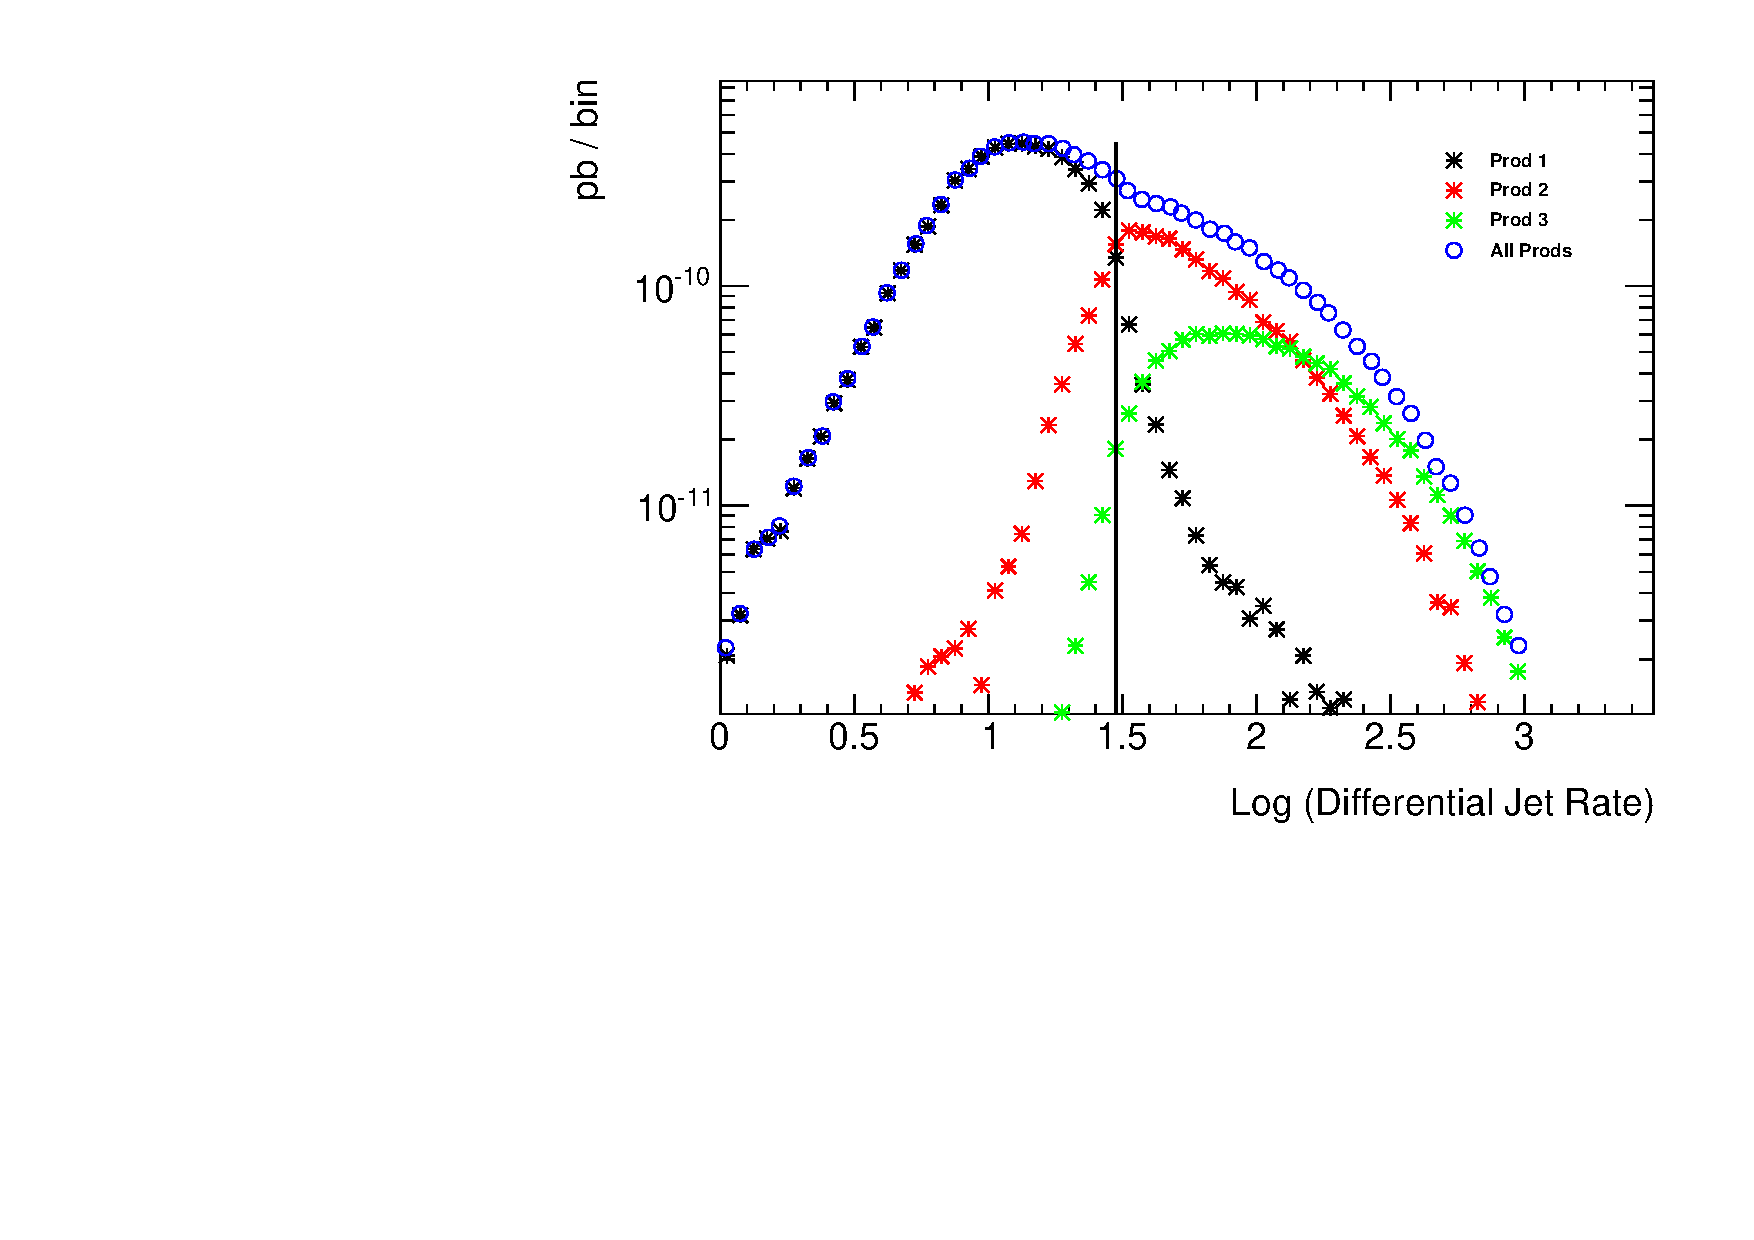
\includegraphics[width=0.45\linewidth]{figures/monojet_appendix/HistoJet1to2_30.pdf}
 	}
 	\hfill
 	\subfloat[$2\rightarrow3$ jets]{%
 		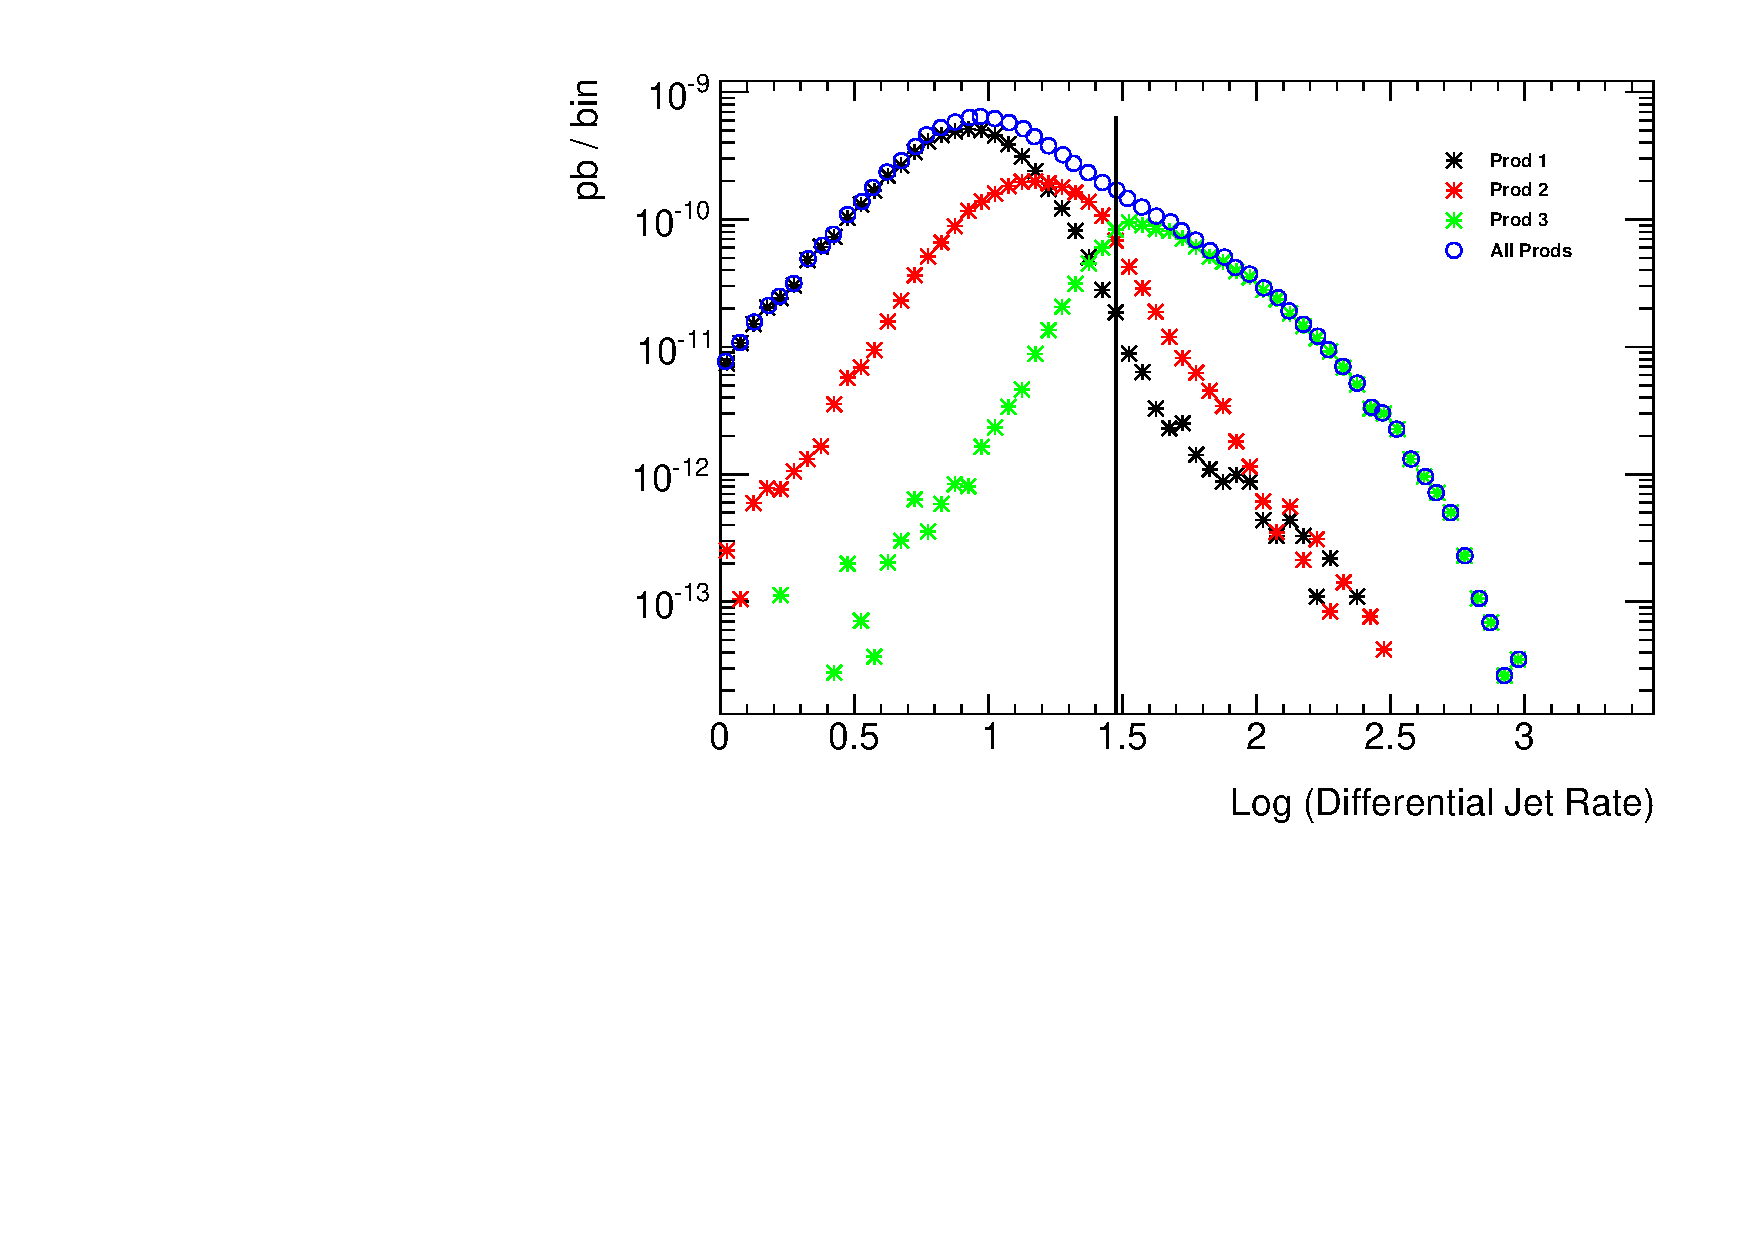
\includegraphics[width=0.45\linewidth]{figures/monojet_appendix/HistoJet2to3_30.pdf}
 	}
 	\hfill
 	\subfloat[$3\rightarrow4$ jets]{%
 		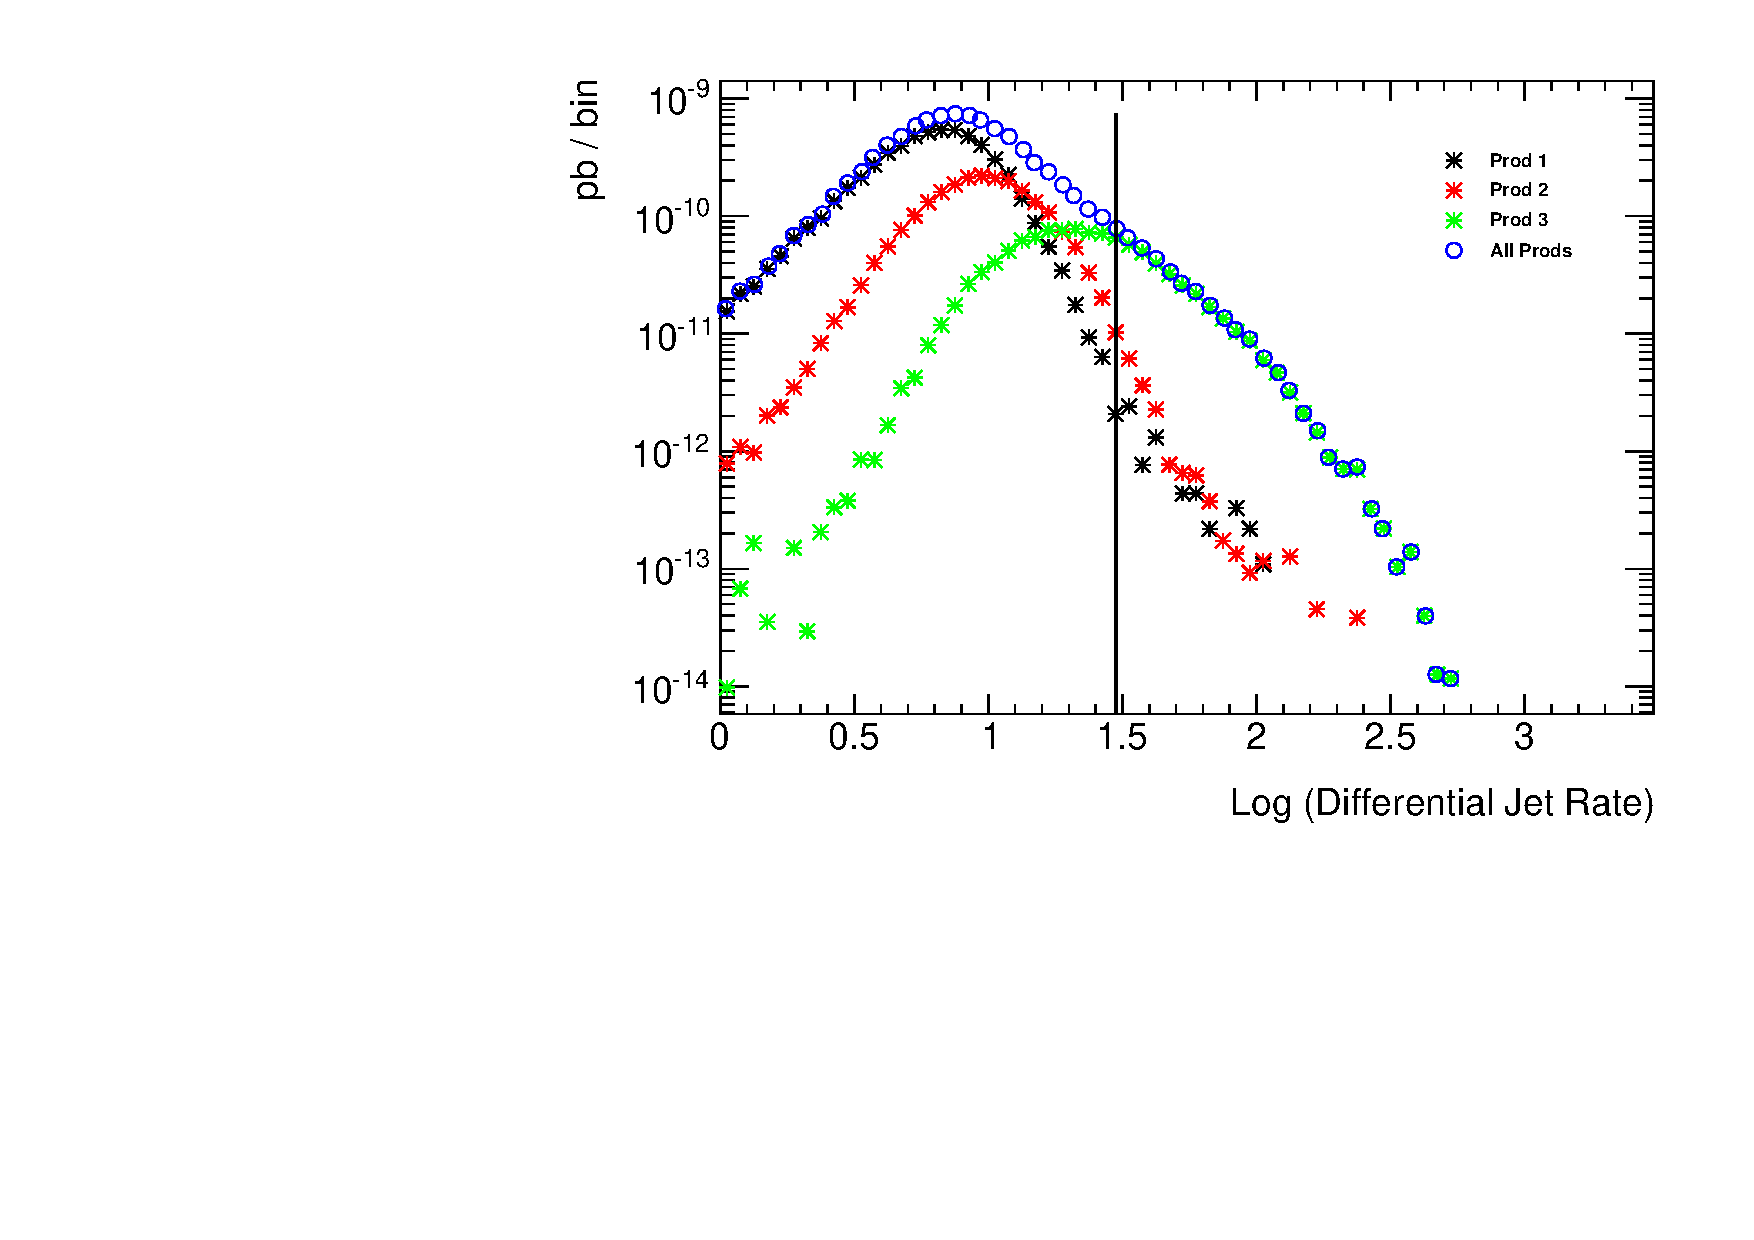
\includegraphics[width=0.45\linewidth]{figures/monojet_appendix/HistoJet3to4_30.pdf}
 	}
 	\hfill
 	\subfloat[$4\rightarrow5$ jets]{%
 		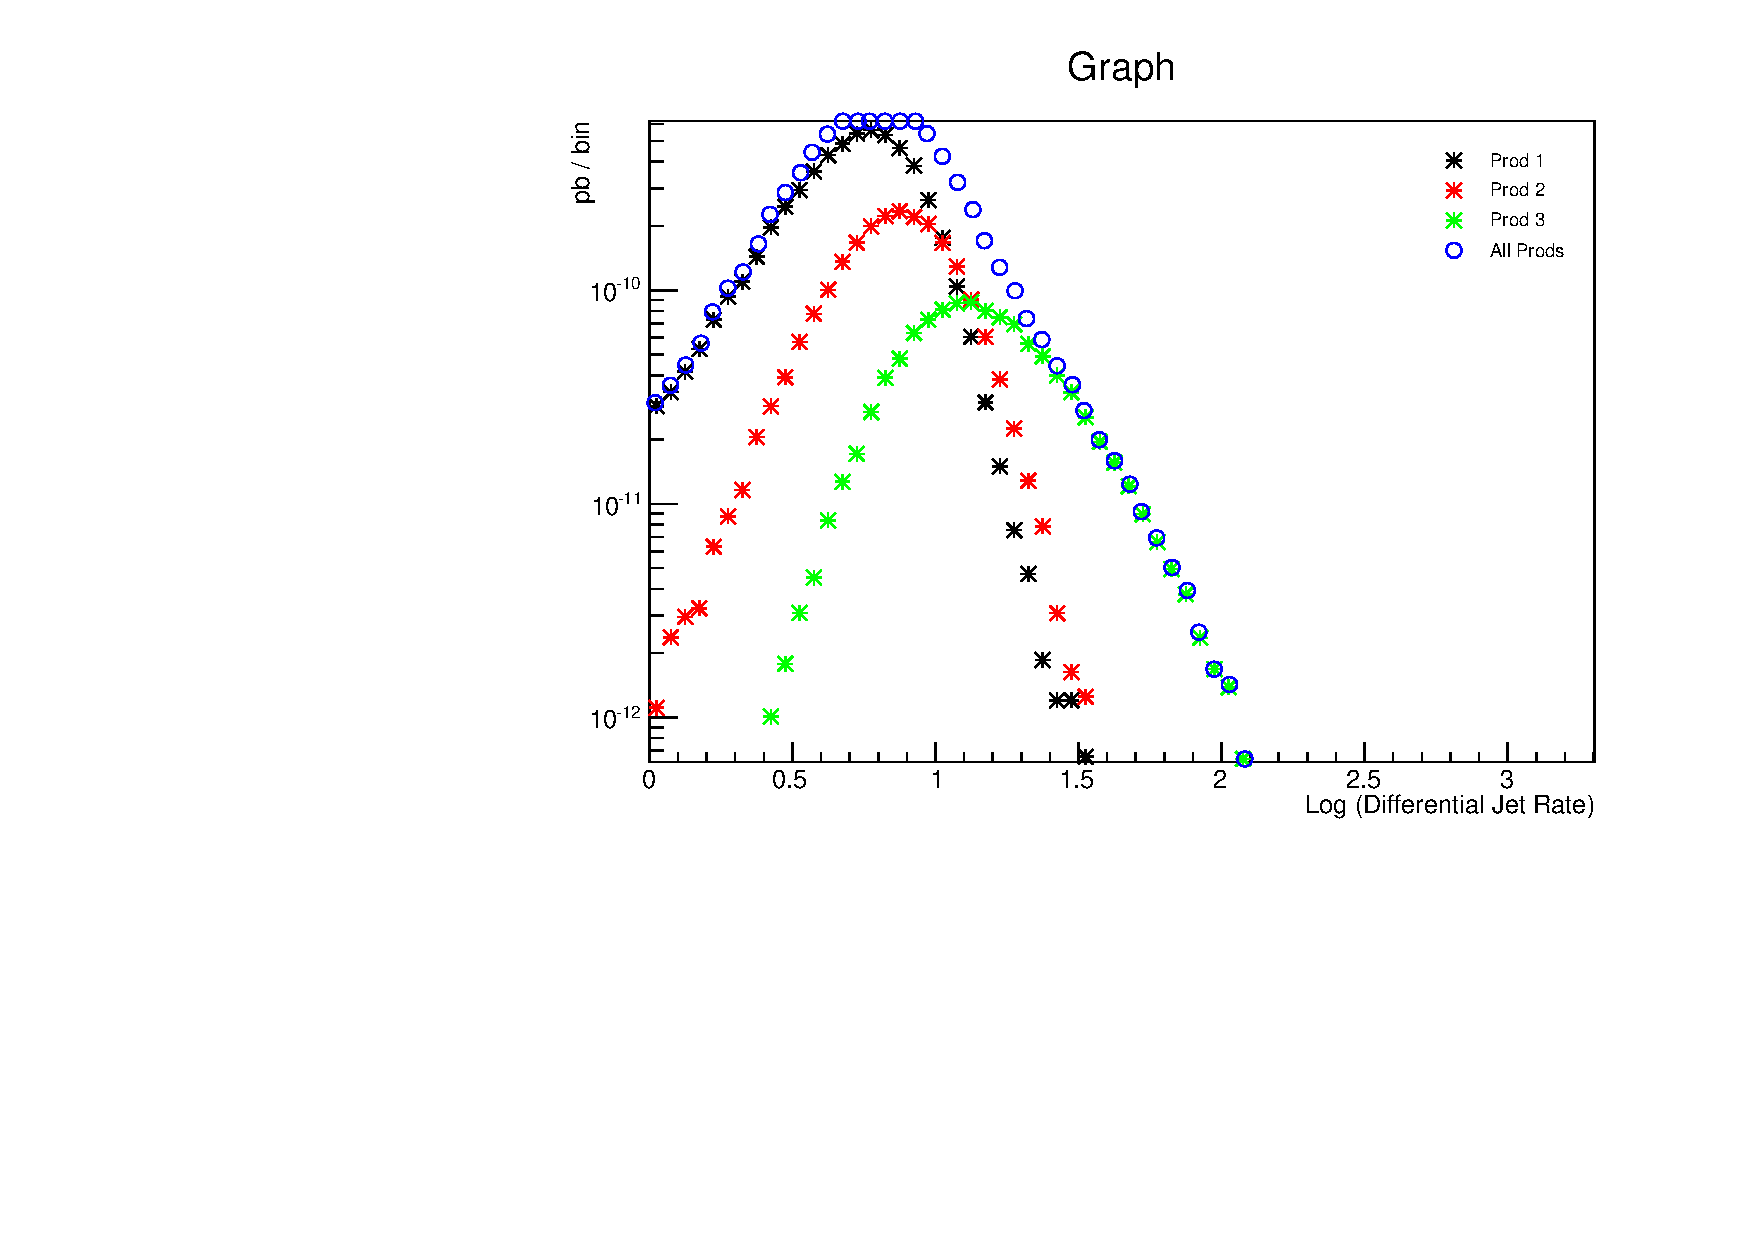
\includegraphics[width=0.45\linewidth]{figures/monojet_appendix/HistoJet4to5_30.pdf}
 	}
 	\caption{Distributions of differential jet rates $\frac{dN_{i\to j}}{d \log_{10}(k_\textrm{cut})}$ for EFT D5 sample with CKKW-L matching scale at 30\,\gev. The 0-, 1- and 2-parton emission samples are generated separately and indicated in the plots as Prod 1, Prod 2 and Prod 3, respectively. A vertical line is drawn at the matching scale.}
 	\label{fig:CKKW_D5_30}
 \end{figure*}


 \begin{figure*}[h!]
 	\centering  
 	\subfloat[$1\rightarrow2$ jets]{%
 		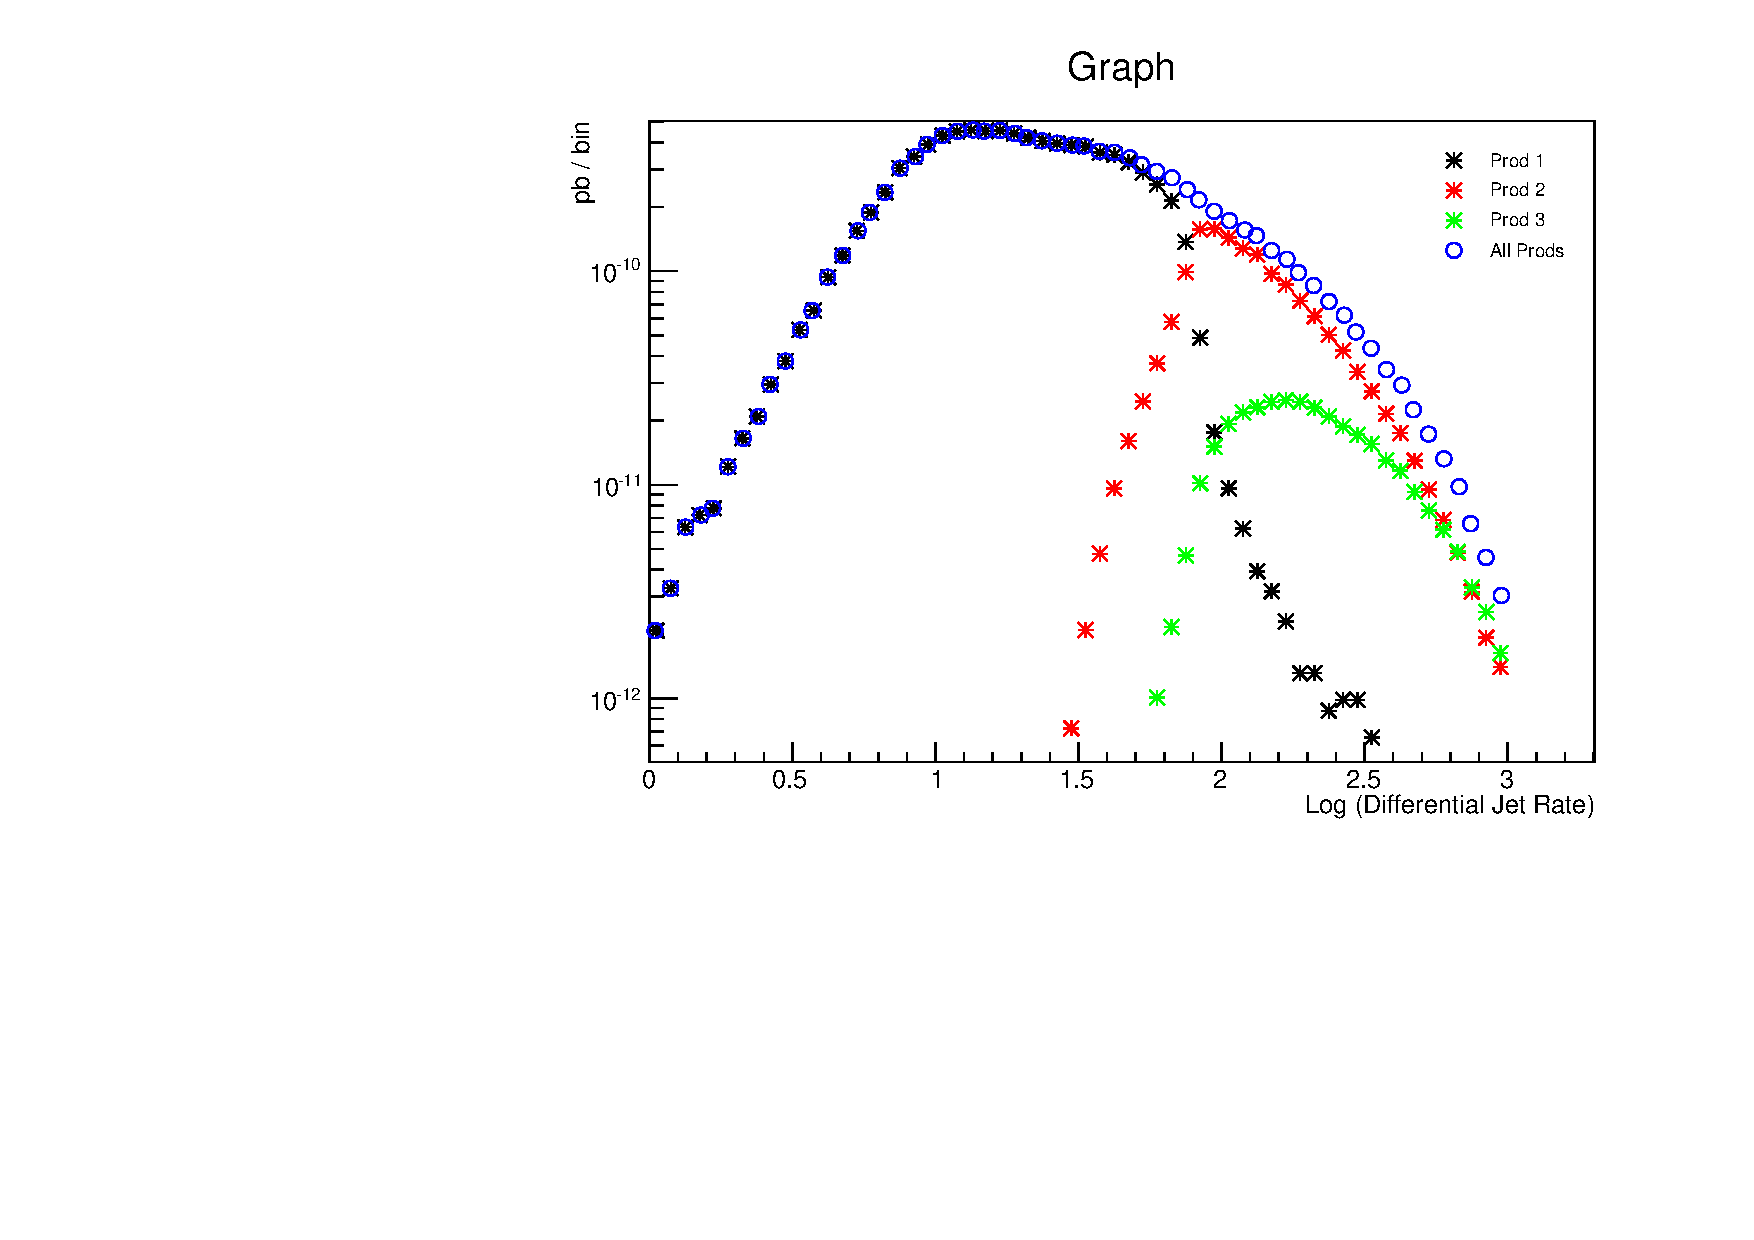
\includegraphics[width=0.45\linewidth]{figures/monojet_appendix/HistoJet1to2_80.pdf}
 	}
 	\hfill
 	\subfloat[$2\rightarrow3$ jets]{%
 		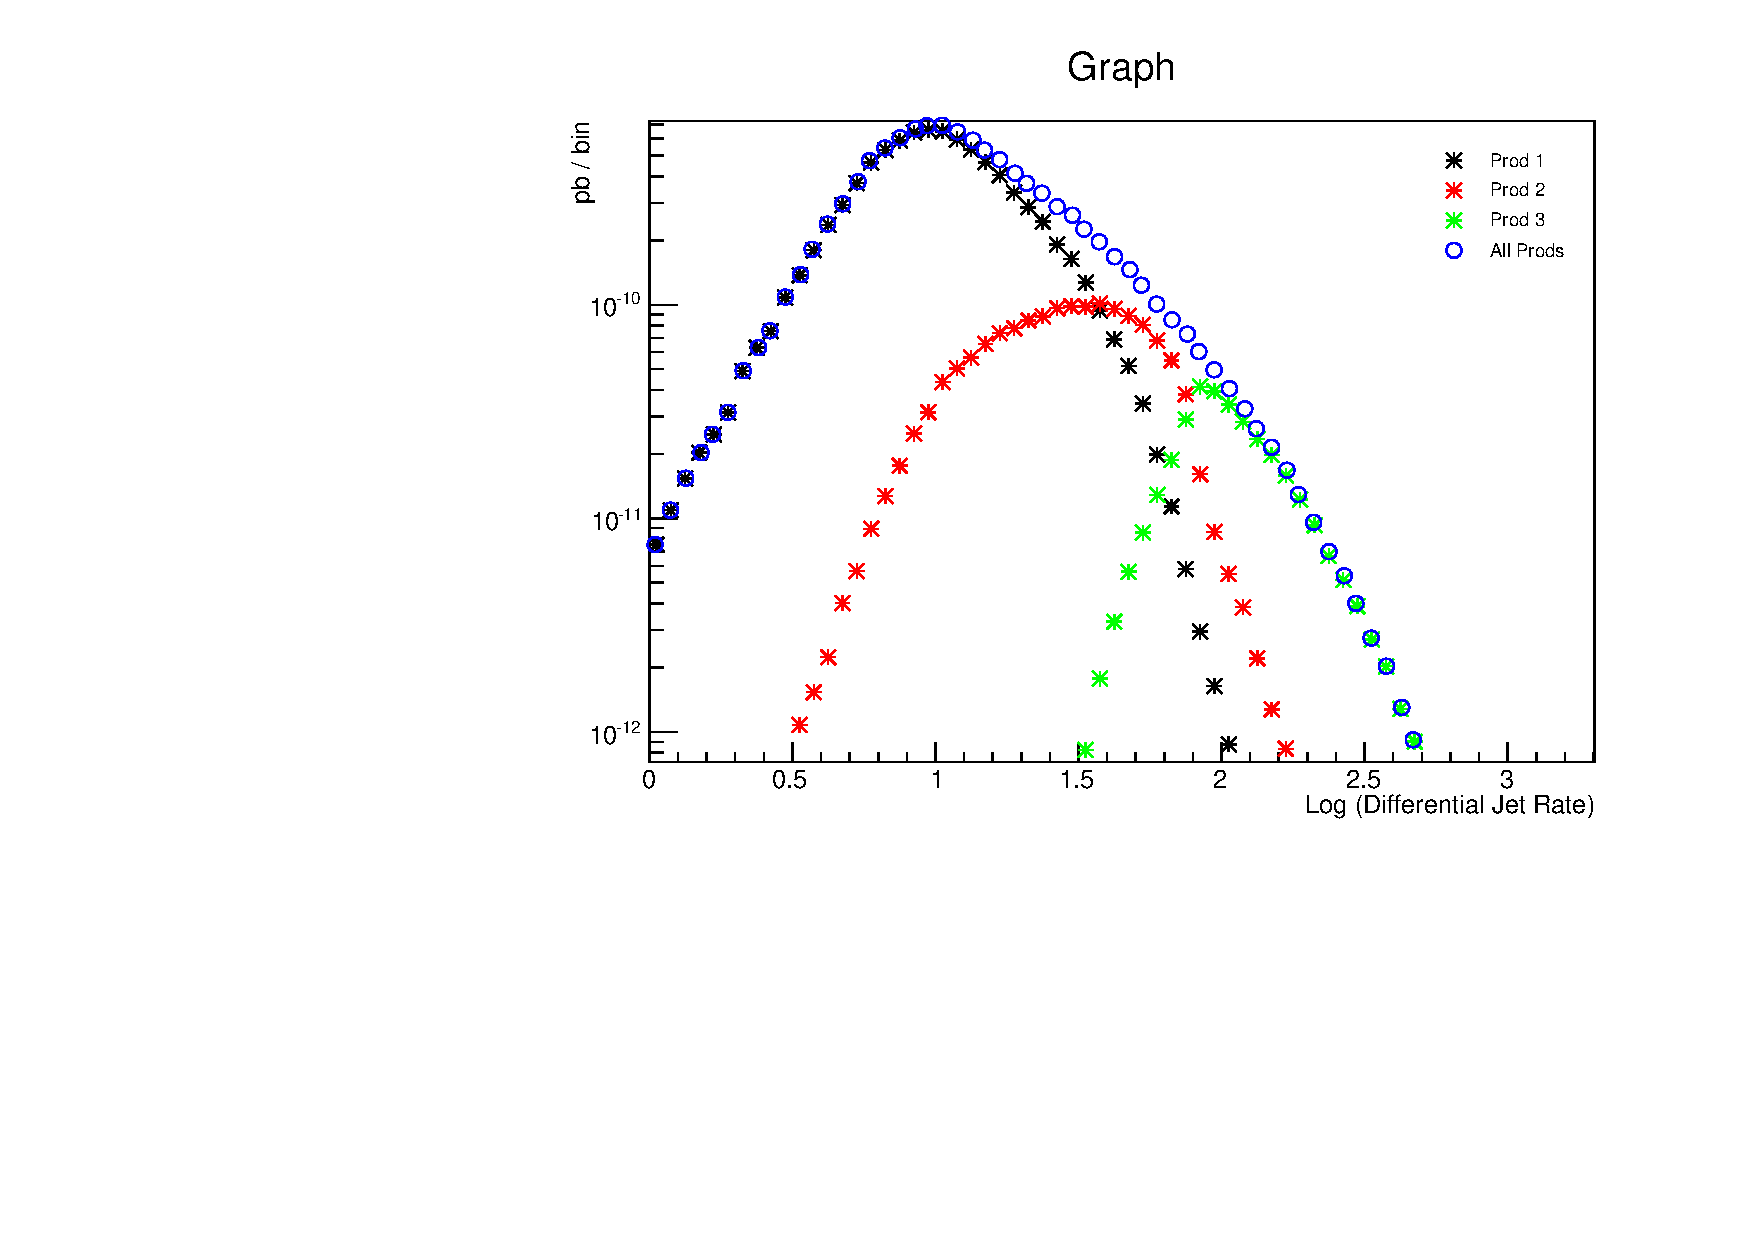
\includegraphics[width=0.45\linewidth]{figures/monojet_appendix/HistoJet2to3_80.pdf}
 	}
 	\hfill
 	\subfloat[$3\rightarrow4$ jets]{%
     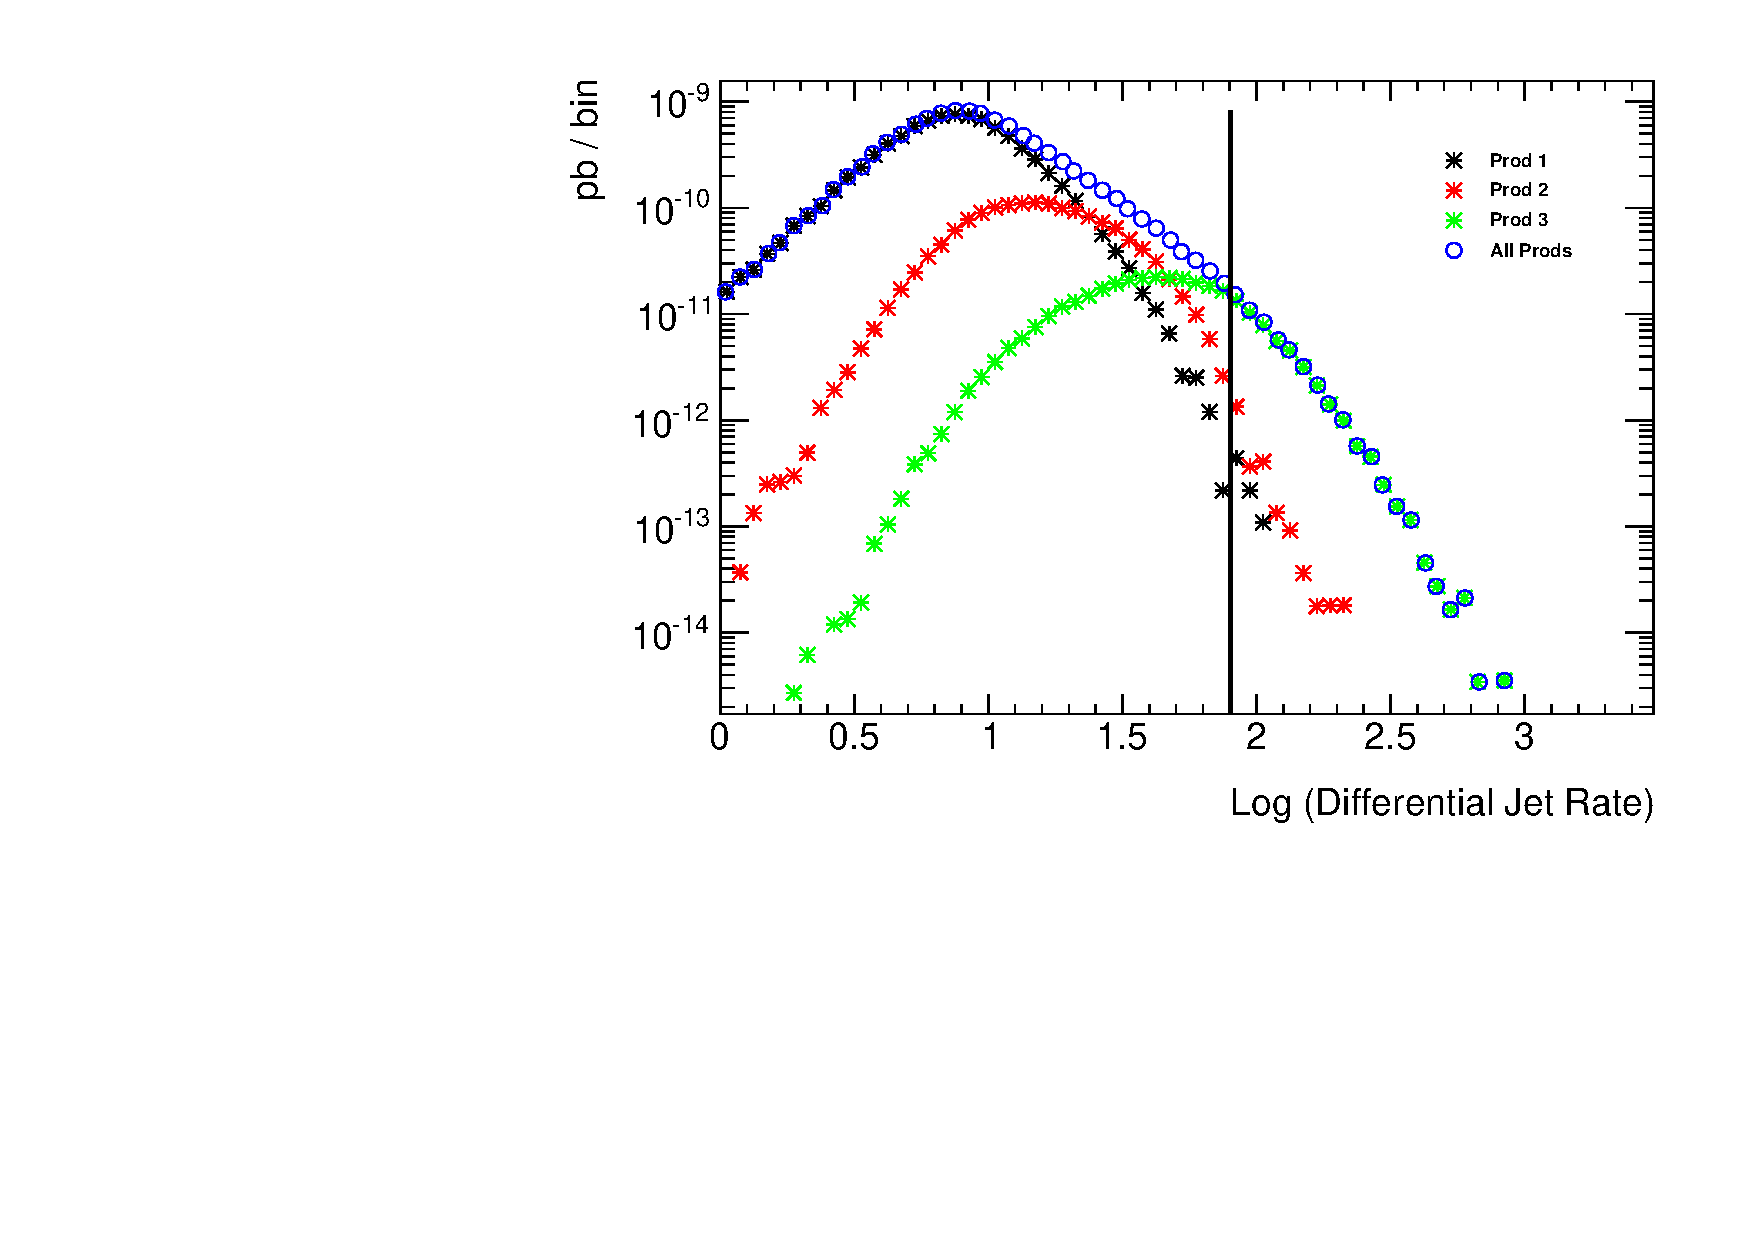
\includegraphics[width=0.45\linewidth]{figures/monojet_appendix/HistoJet3to4_80.pdf}
 	}
 	\hfill
 	\subfloat[$4\rightarrow5$ jets]{%
     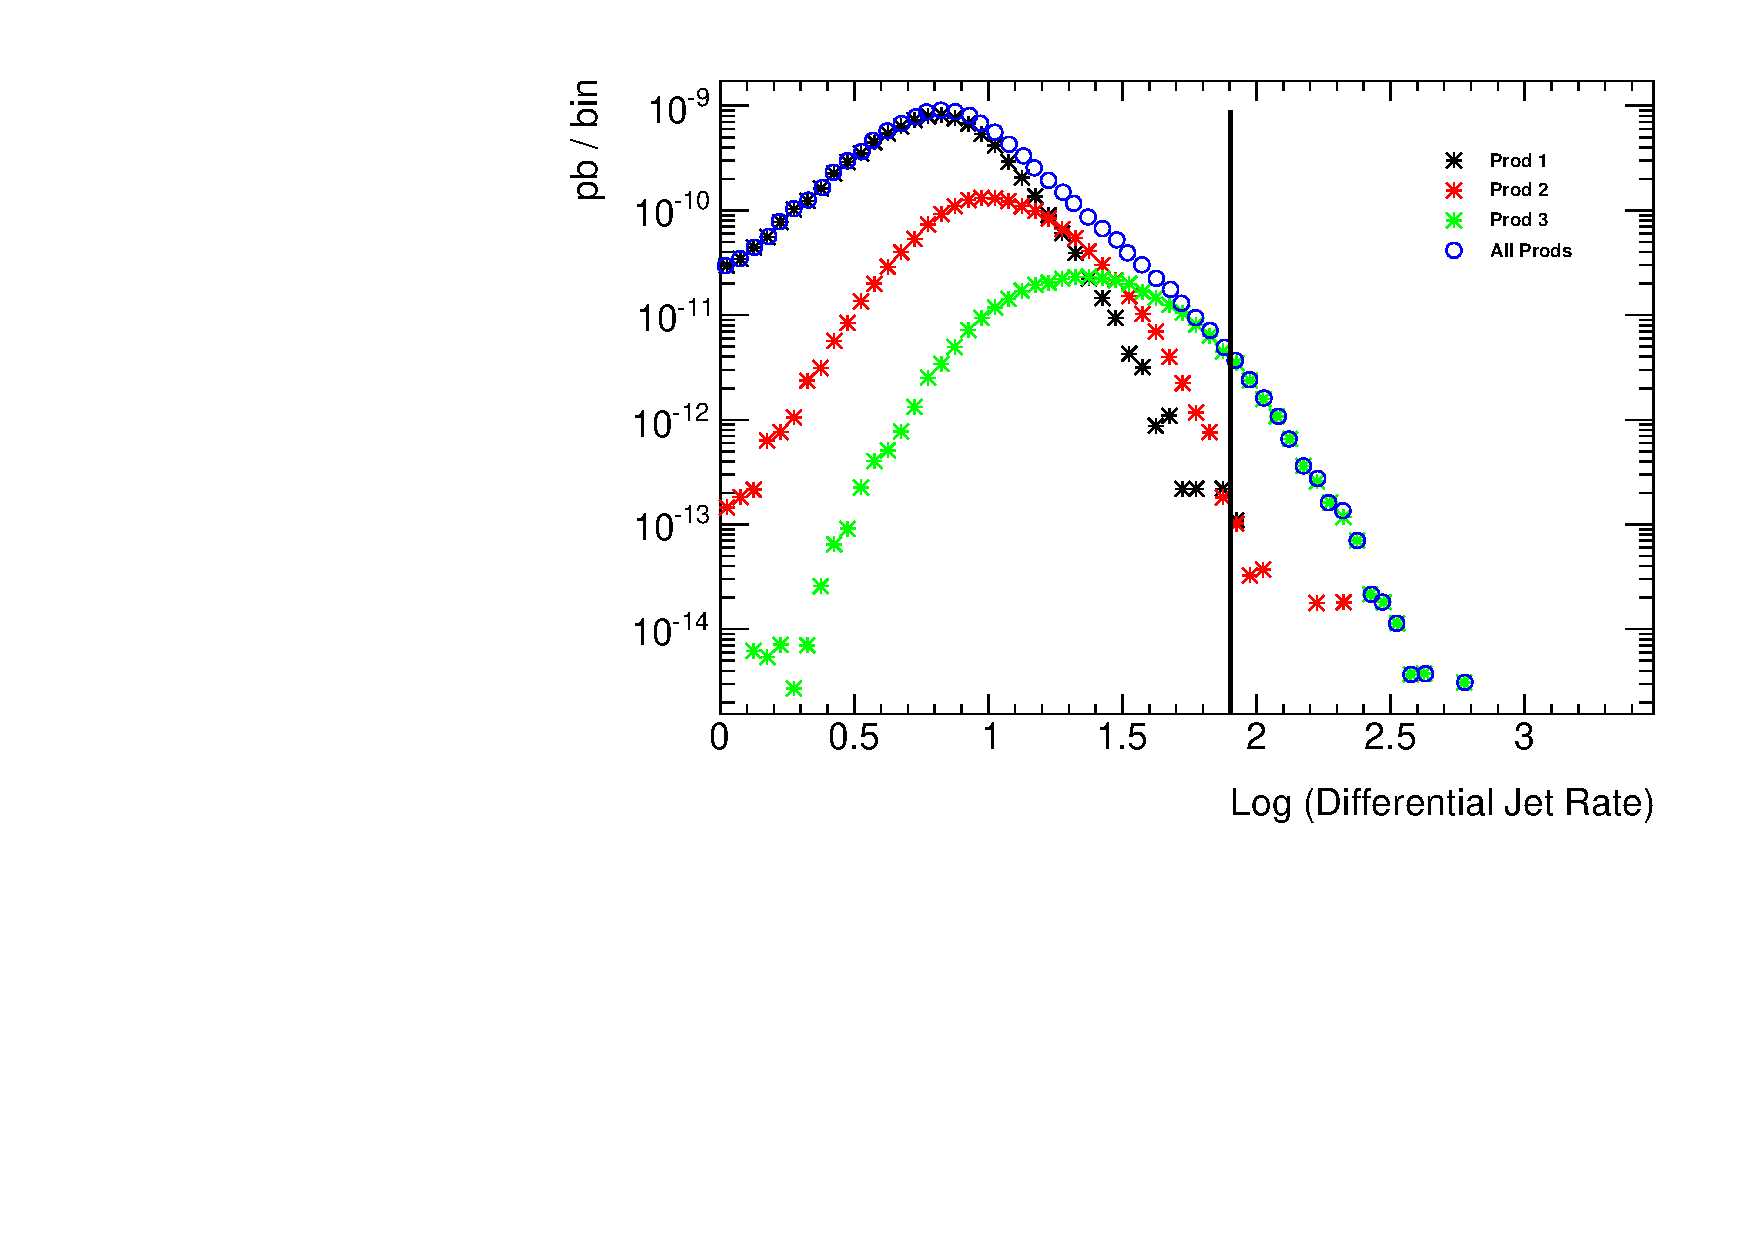
\includegraphics[width=0.45\linewidth]{figures/monojet_appendix/HistoJet4to5_80.pdf}
 	}
   \caption{Distributions of differential jet rates $\frac{dN_{i\to j}}{d \log_{10}(k_\textrm{cut})}$ for EFT D5 sample with CKKW-L matching scale at 80\,\gev. The 0-, 1- and 2-parton emission samples are generated separately and indicated in the plots as Prod 1, Prod 2 and Prod 3, respectively. A vertical line is drawn at the matching scale.}
   \label{fig:CKKW_D5_80}
 \end{figure*}


 \begin{figure*}[h!]
 	\centering  
 	\subfloat[$1\rightarrow2$ jets]{%
 		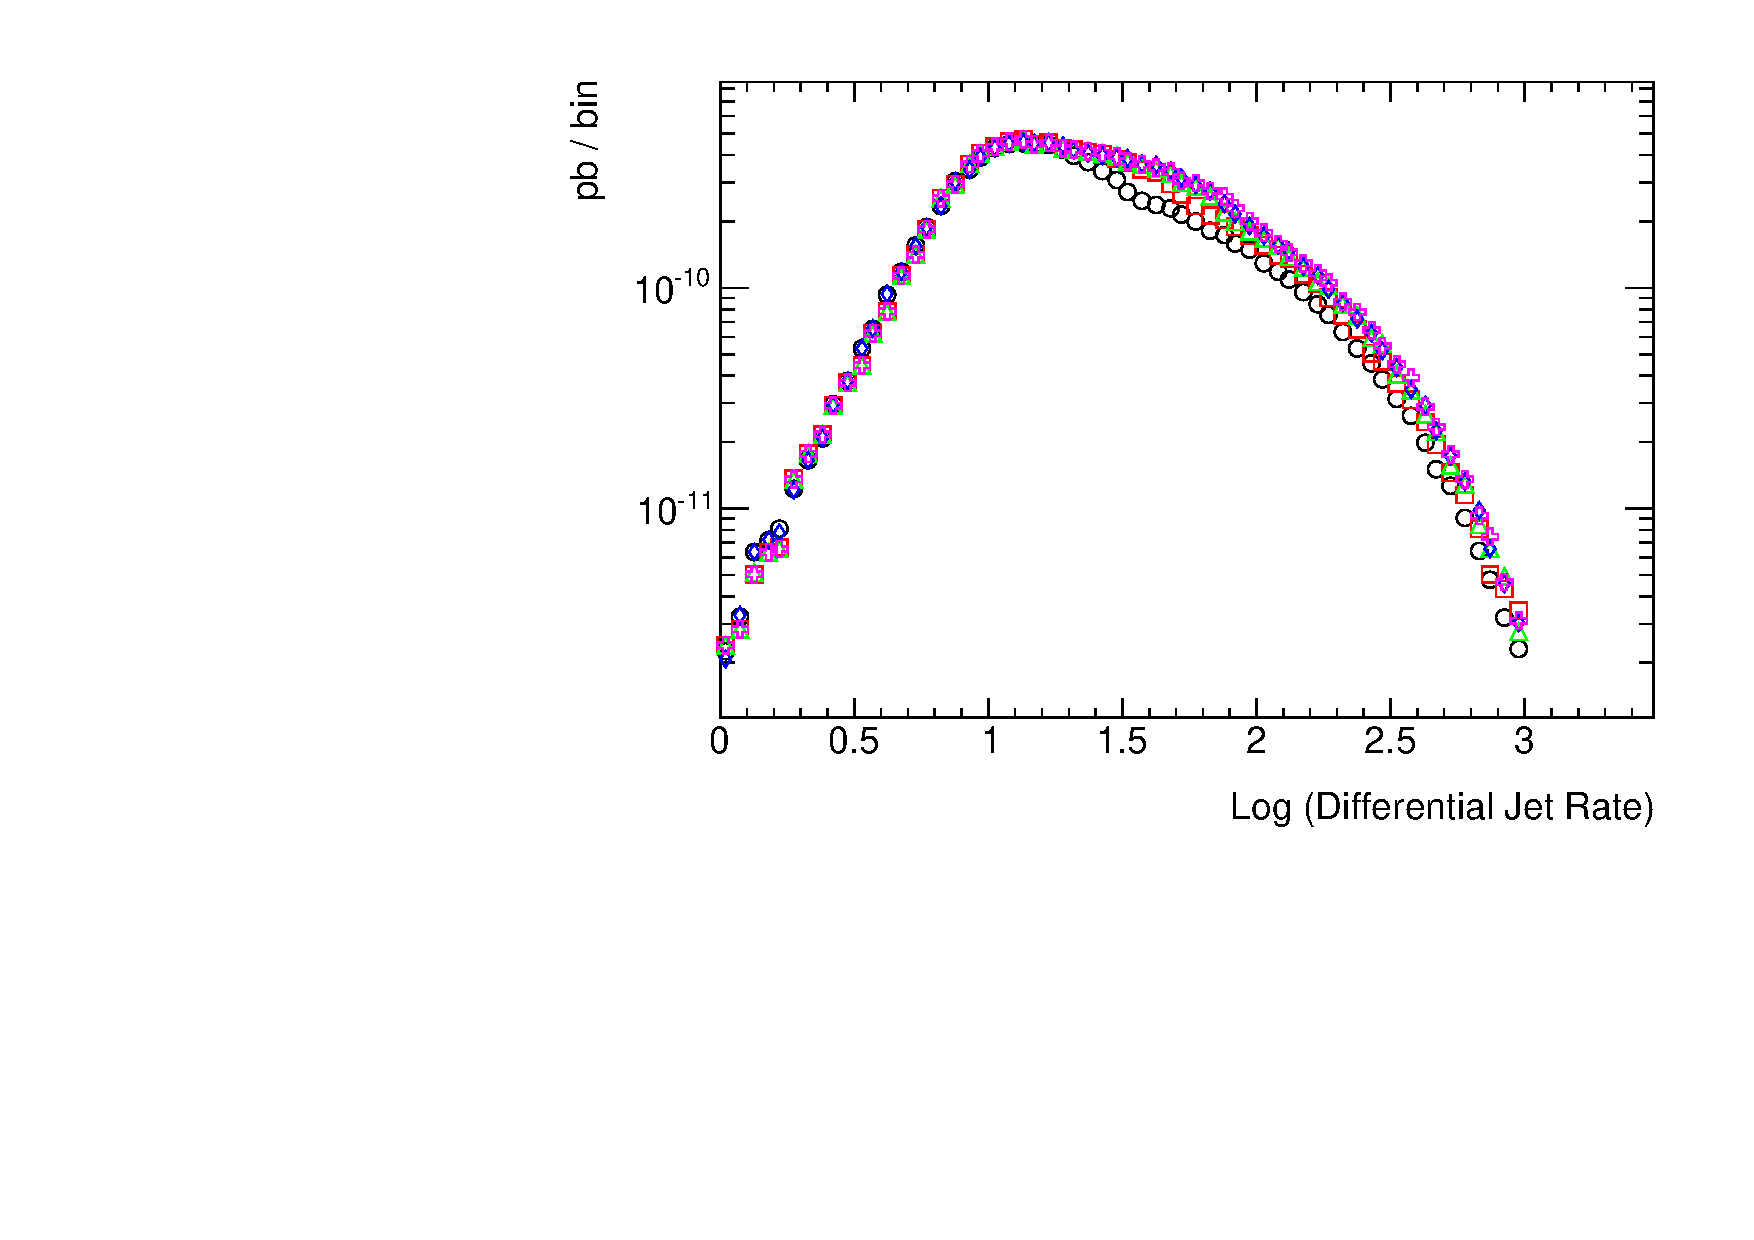
\includegraphics[width=0.45\linewidth]{figures/monojet_appendix/compare_plot_1.pdf}
 		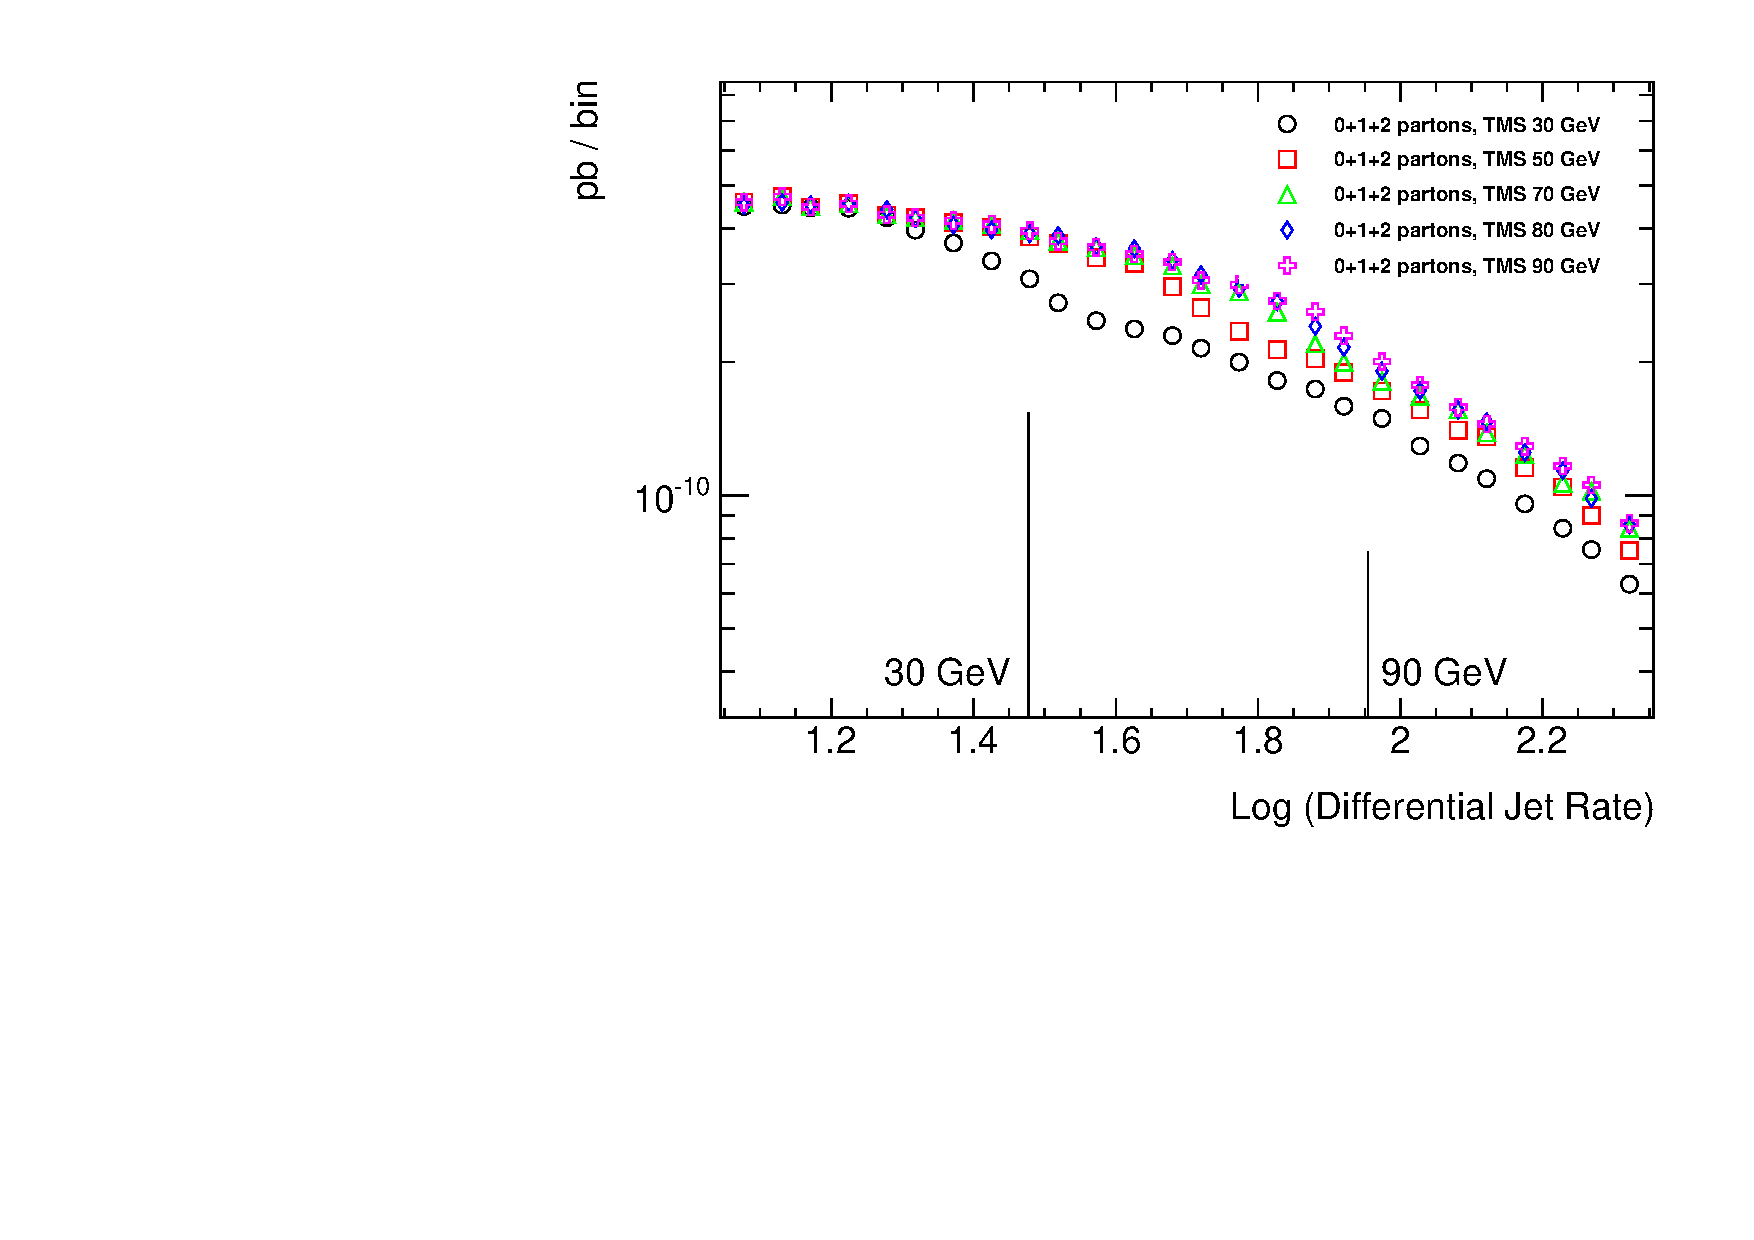
\includegraphics[width=0.45\linewidth]{figures/monojet_appendix/window_plot_1.pdf}
 	}
 	\hfill
 	\subfloat[$2\rightarrow3$ jets]{%
 		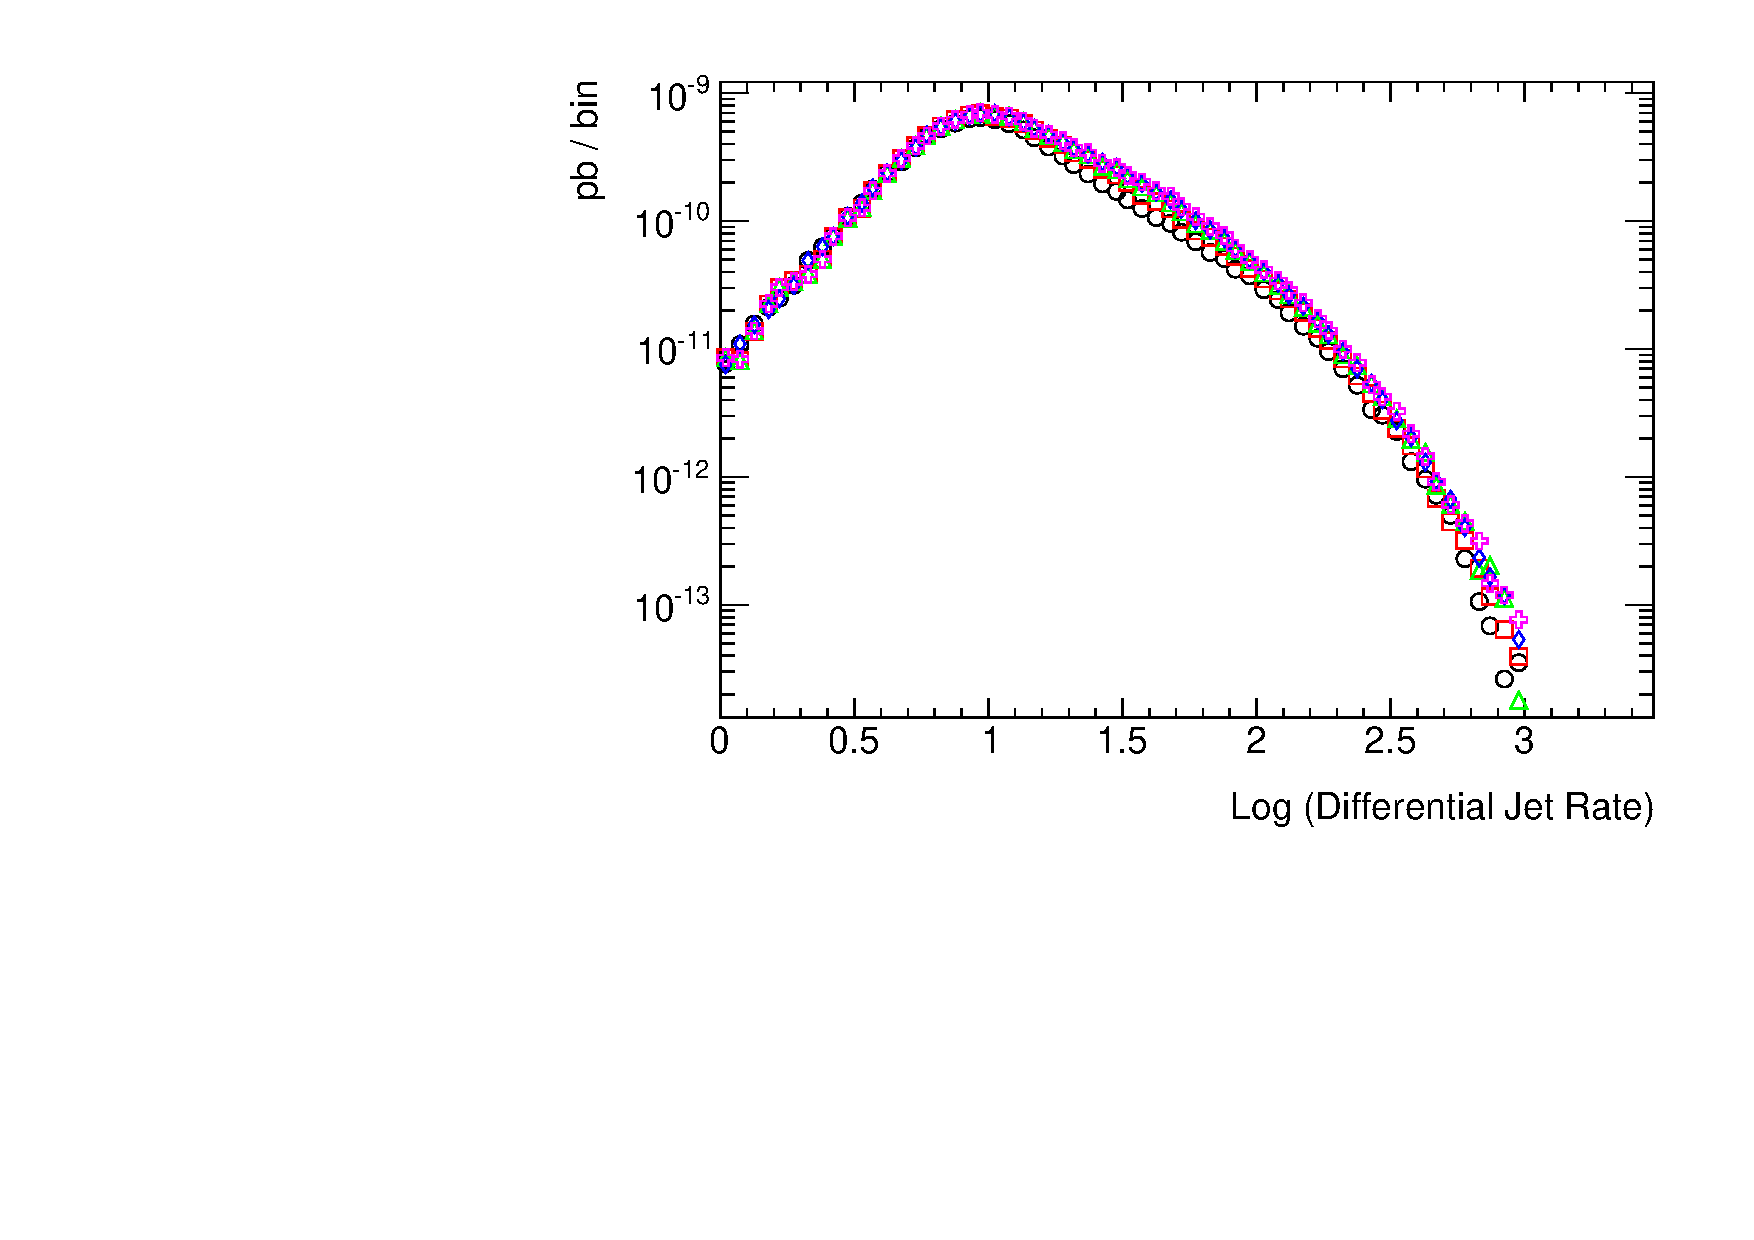
\includegraphics[width=0.45\linewidth]{figures/monojet_appendix/compare_plot_2.pdf}
 		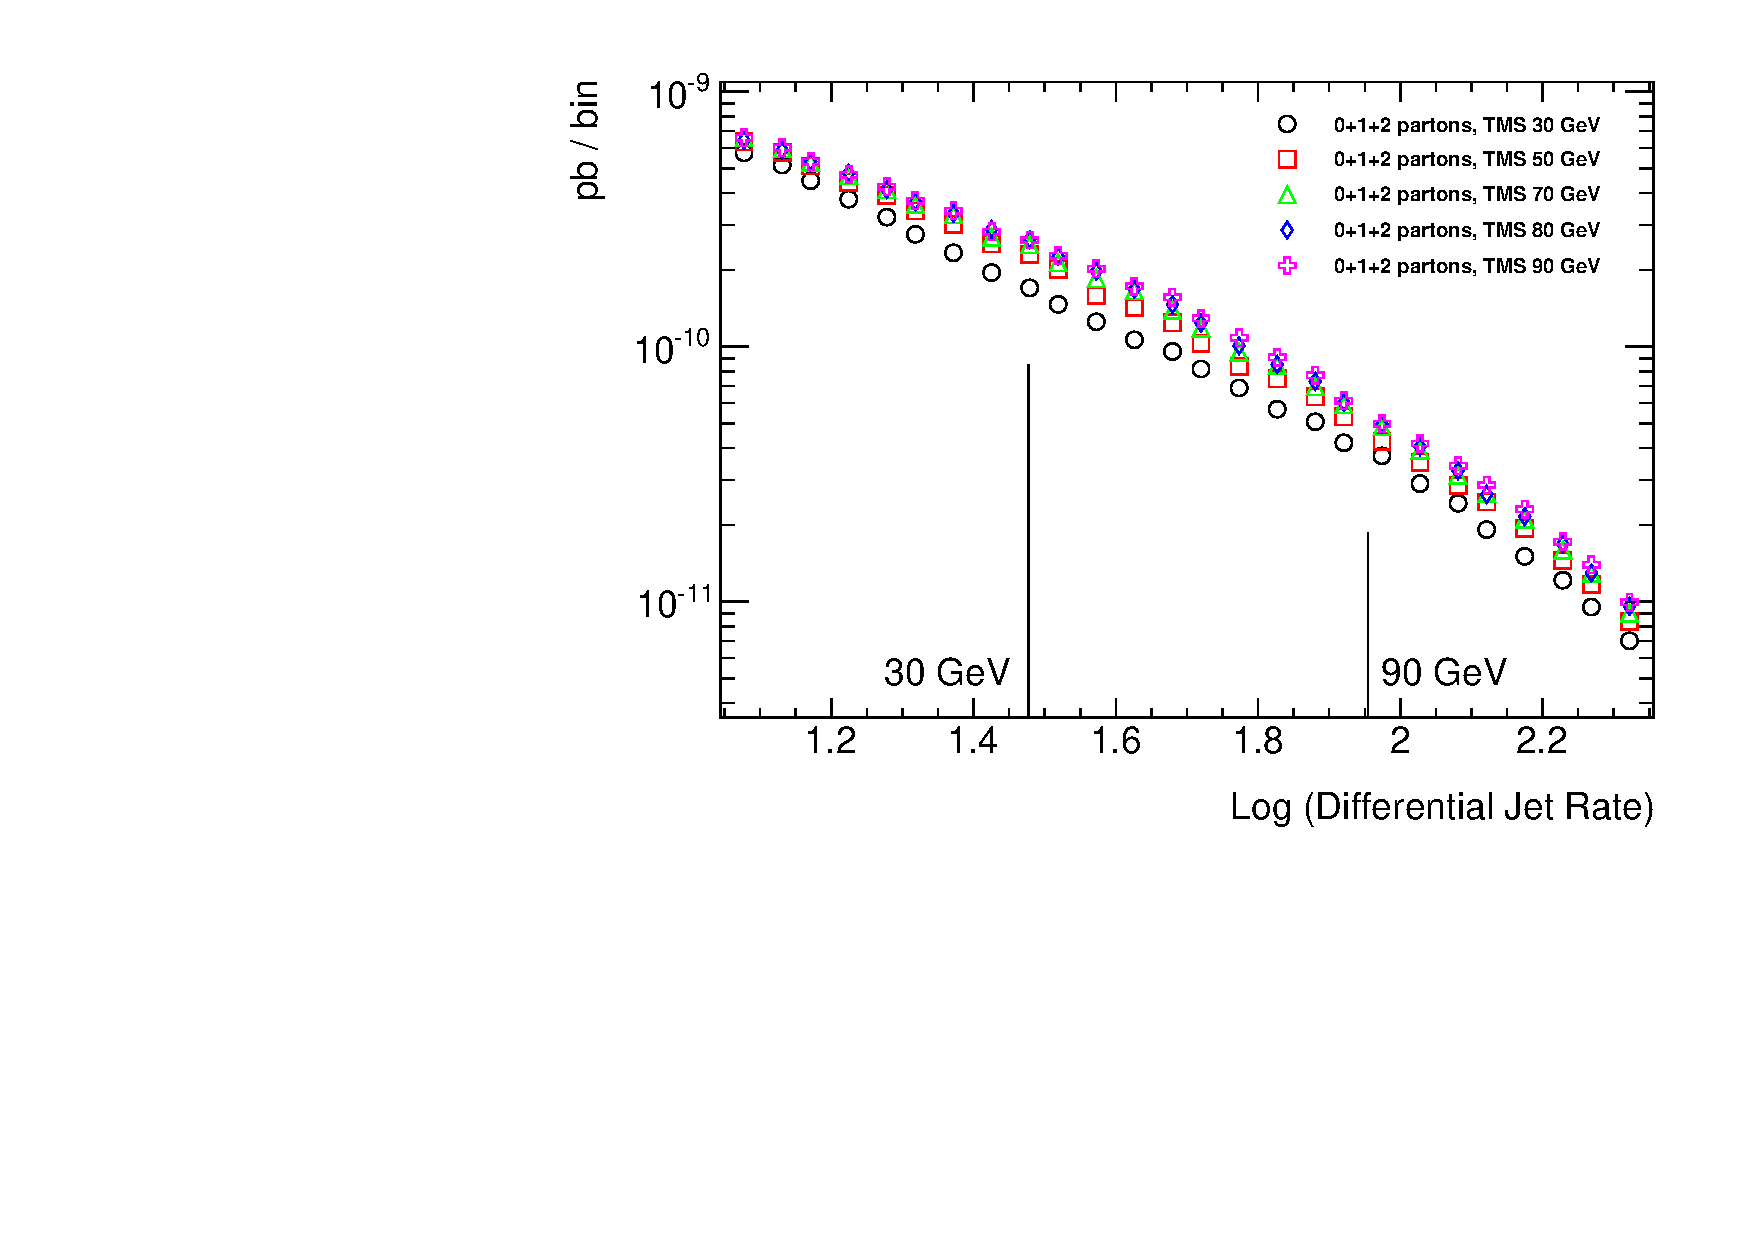
\includegraphics[width=0.45\linewidth]{figures/monojet_appendix/window_plot_2.pdf}
 	}
 	\hfill
 	\subfloat[$3\rightarrow4$ jets]{%
 		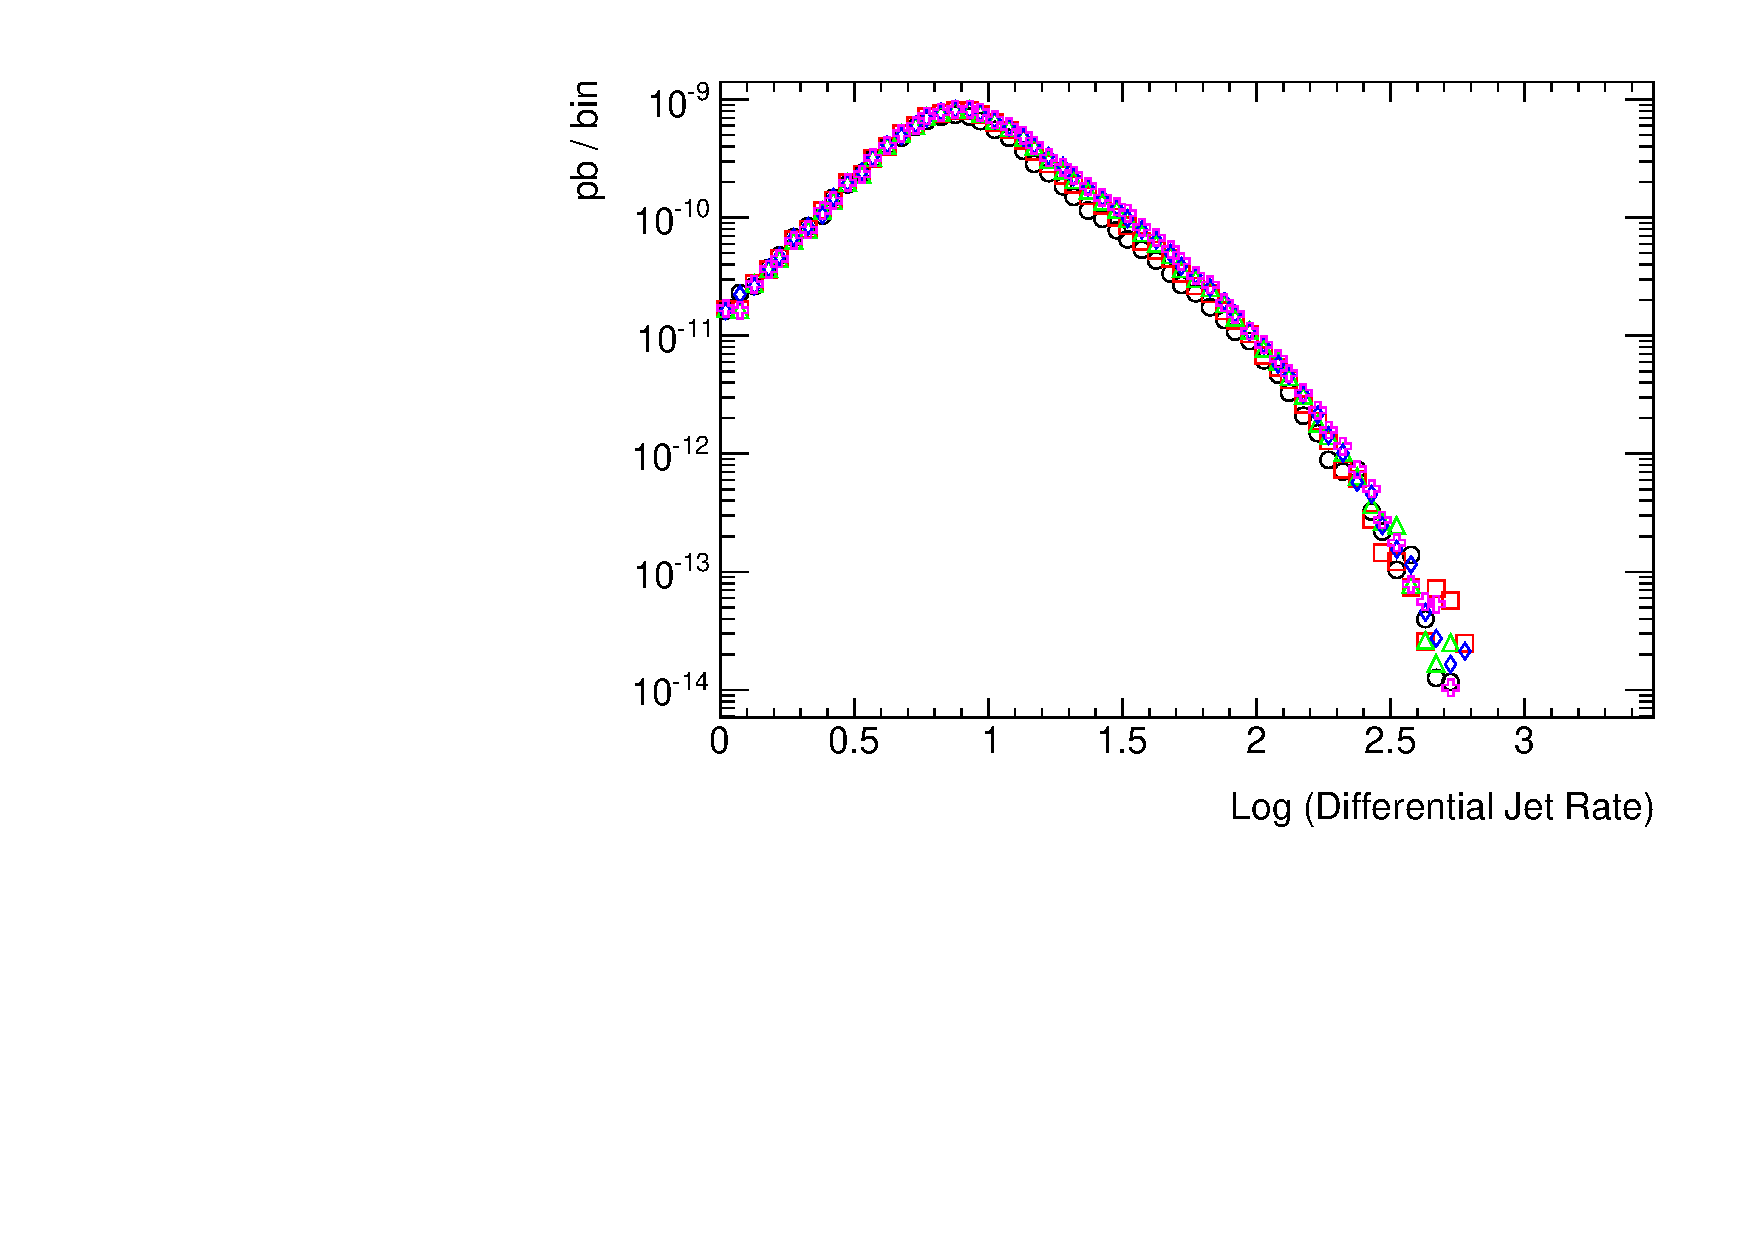
\includegraphics[width=0.45\linewidth]{figures/monojet_appendix/compare_plot_3.pdf}
 		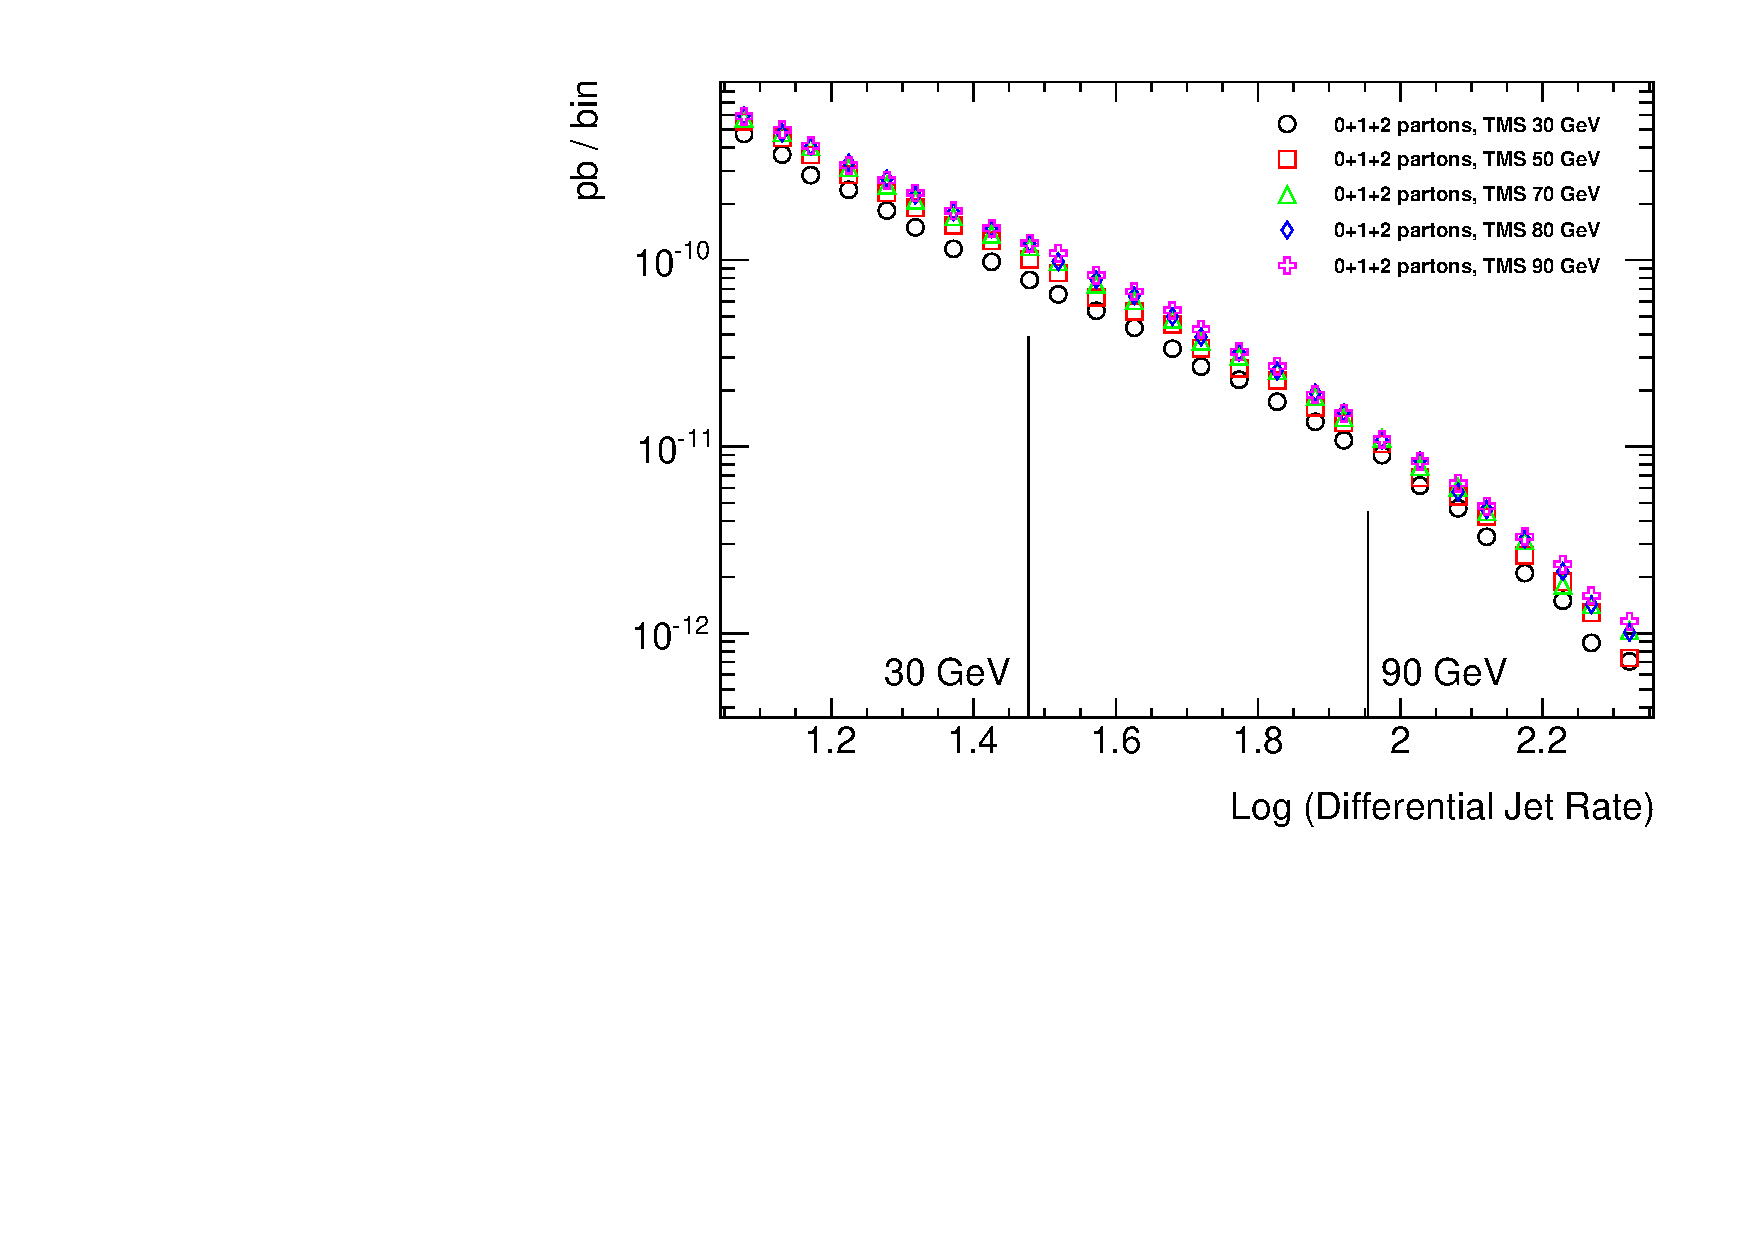
\includegraphics[width=0.45\linewidth]{figures/monojet_appendix/window_plot_3.pdf}
 	}
 	\hfill
 	\subfloat[$4\rightarrow5$ jets]{%
 		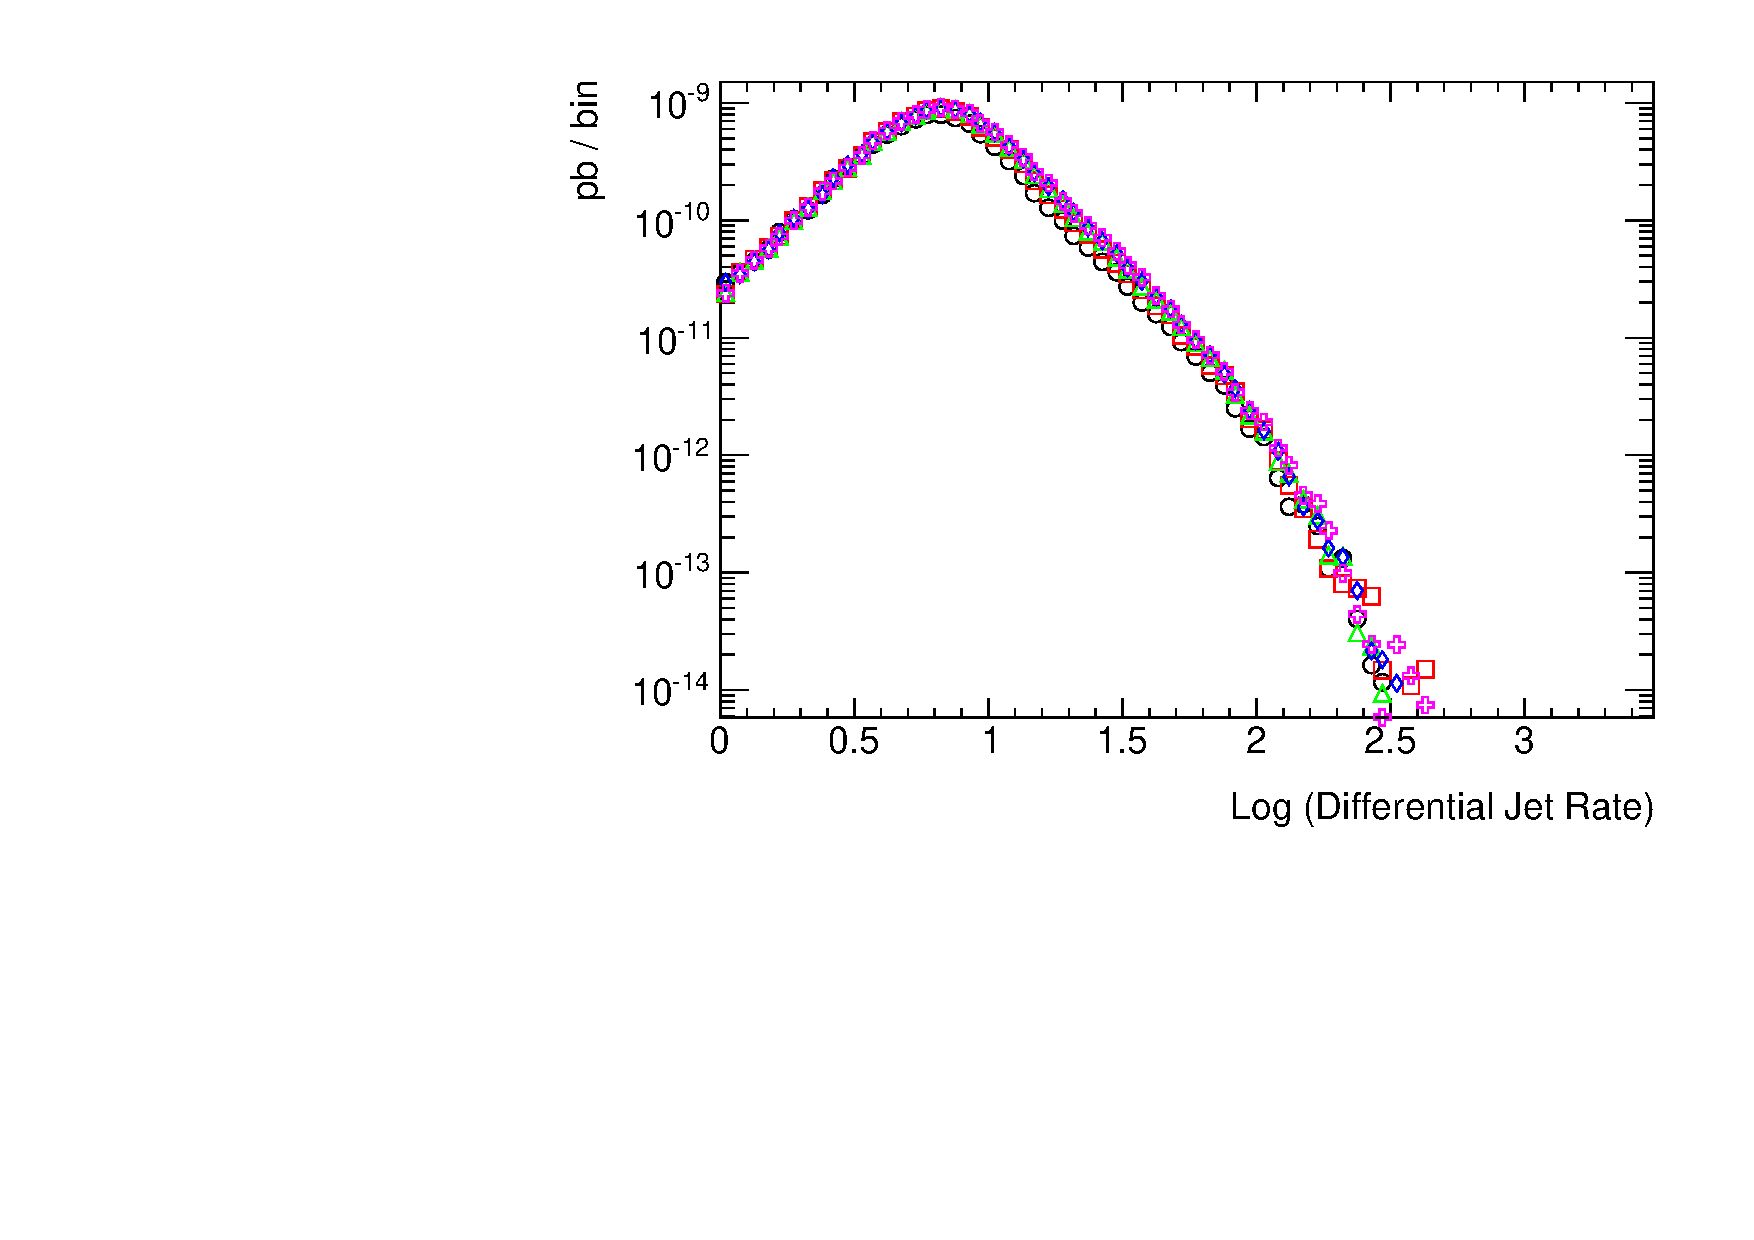
\includegraphics[width=0.45\linewidth]{figures/monojet_appendix/compare_plot_4.pdf}
 		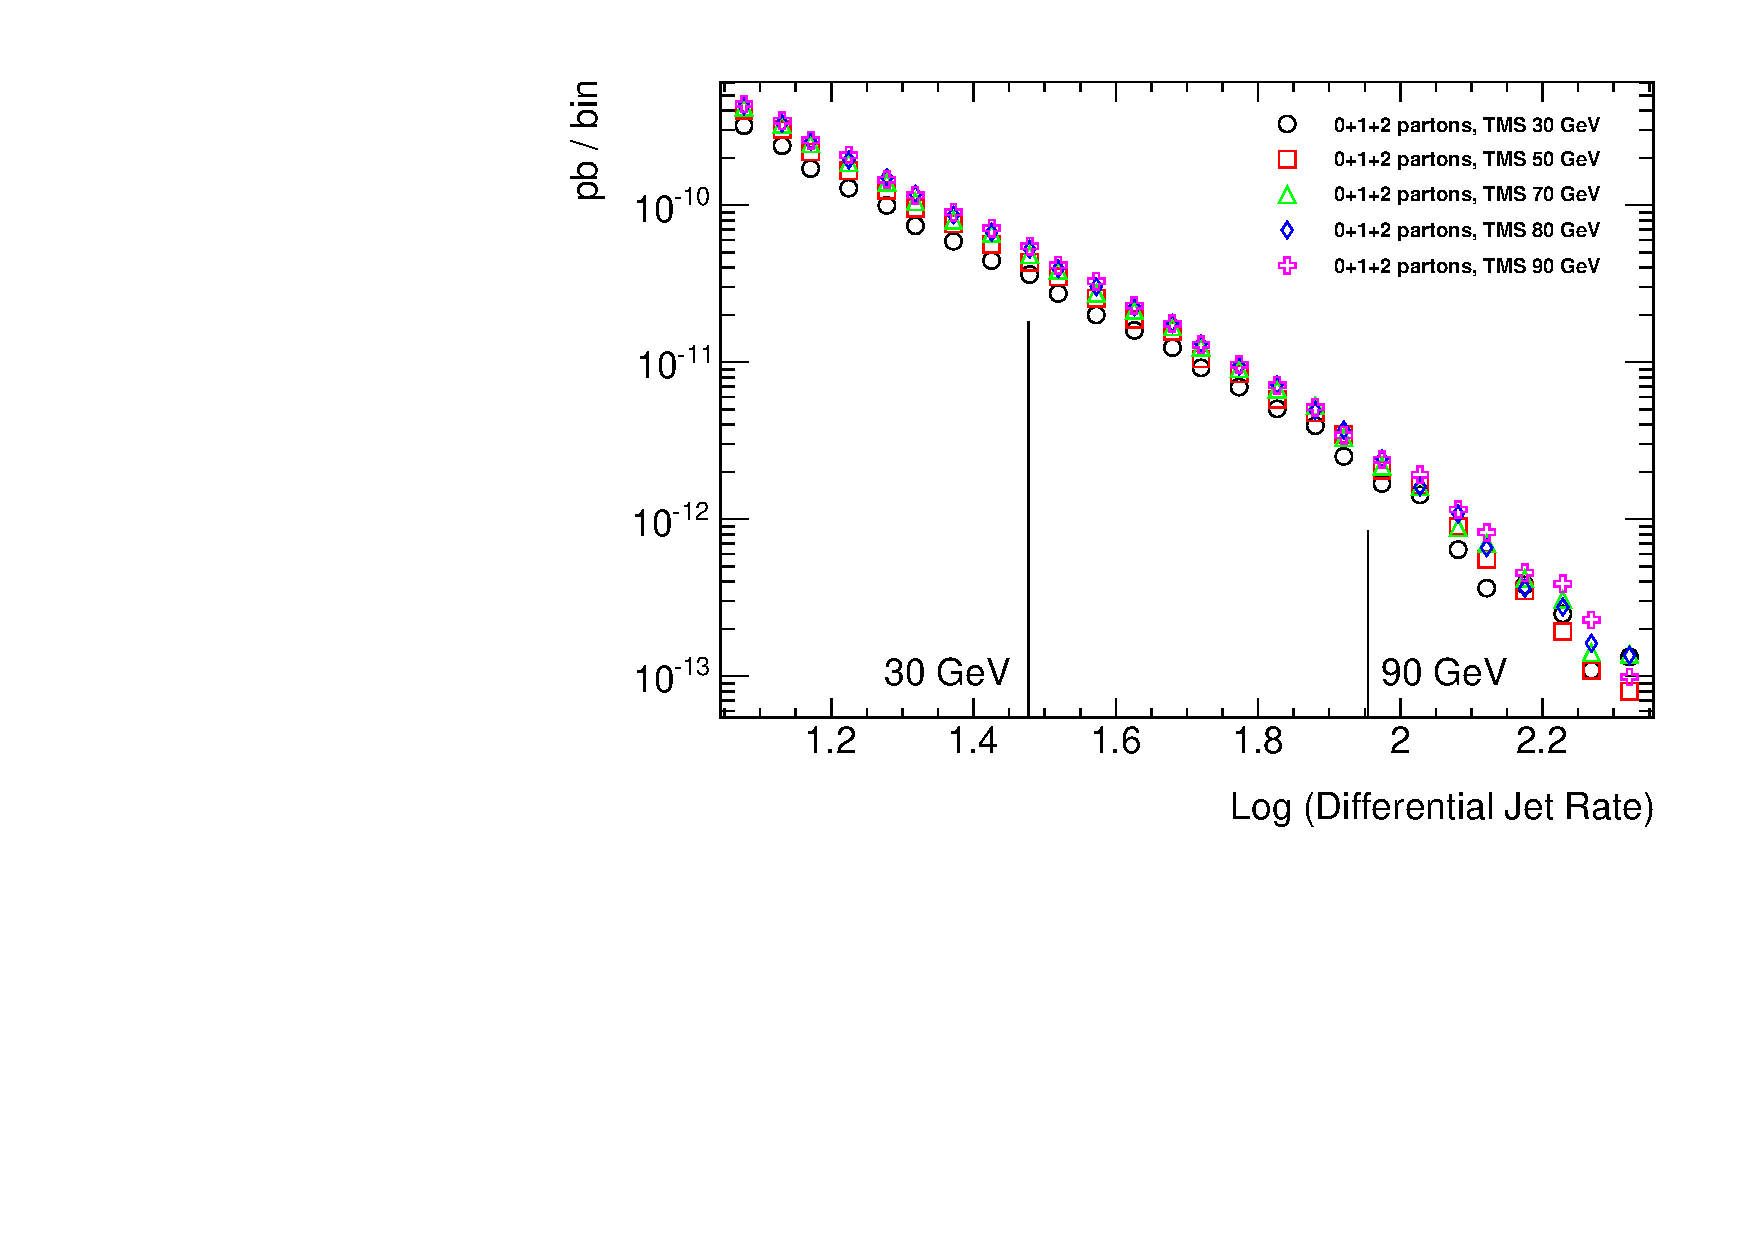
\includegraphics[width=0.45\linewidth]{figures/monojet_appendix/window_plot_4.pdf}
 	}
   \caption{Distributions of differential jet rates $\frac{dN_{i\to j}}{d \log_{10}(k_\textrm{cut})}$ for EFT D5 sample with CKKW-L matching scale at 30, 50, 70, 80 and 90\,\gev. A zoom of the region around the matching scale values is shown on right.}
   \label{fig:CKKW_D5_zoom}
 \end{figure*}


%% \subsubsection{Parton emission multiplicity}
%% \label{sec:monojet_parton_emission}

 The prescription for the event generation given in Section\,\ref{sec:match_implementation} starts with the emission of 0 partons and ends with maxim 2 partons in addition. Producing the samples separately allows to investigate the relative composition of the individual samples in various parts of the phase space. Figure\,\ref{fig:Kine_D5_80} shows the \MET distribution of the EFT D5 sample with the matching scale at 80\,\gev. The plot reveals that the 0-parton sample gives the dominant contribution in the region below the matching scale value that rapidly decreases at higher \MET. Assuming the lowest analysis \MET cut in early Run-2 mono-jet analyses at 300\,\gev, the generation of the 0-parton emission sample can be safely omitted as it only gives $<1\%$ contribution at $\MET>300\,\gev$. For the 1- and 2-parton emission samples, one can use a generator cut on the leading parton $\pT$, \texttt{ptj1min}, in order to avoid generating low \MET events that are irrelevant for the analysis.

 \begin{figure}[h!]
 	\centering  
 %	\subfloat[Missing transverse momentum]{%
     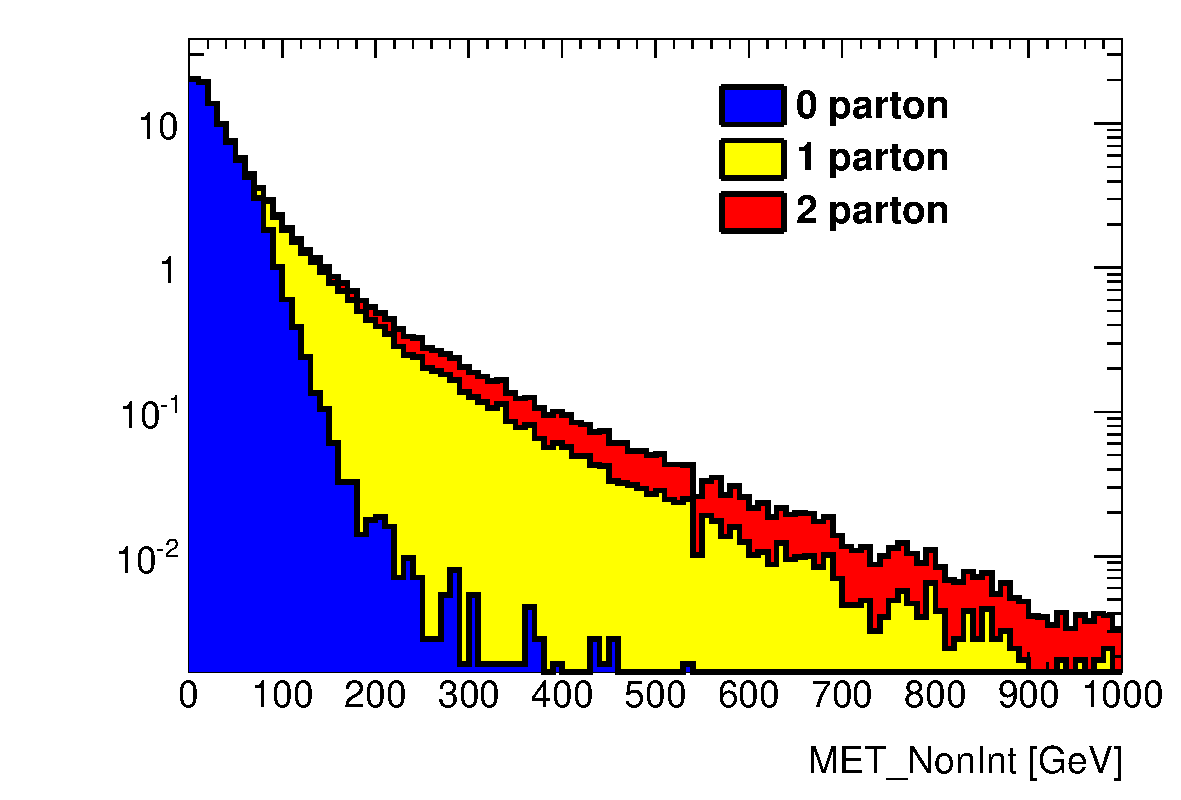
\includegraphics[width=0.95\linewidth]{figures/monojet_appendix/MET_matching80.pdf}
 %	}
 %	\hfill
 %	\subfloat[Transverse momentum of leading jet]{%
 %    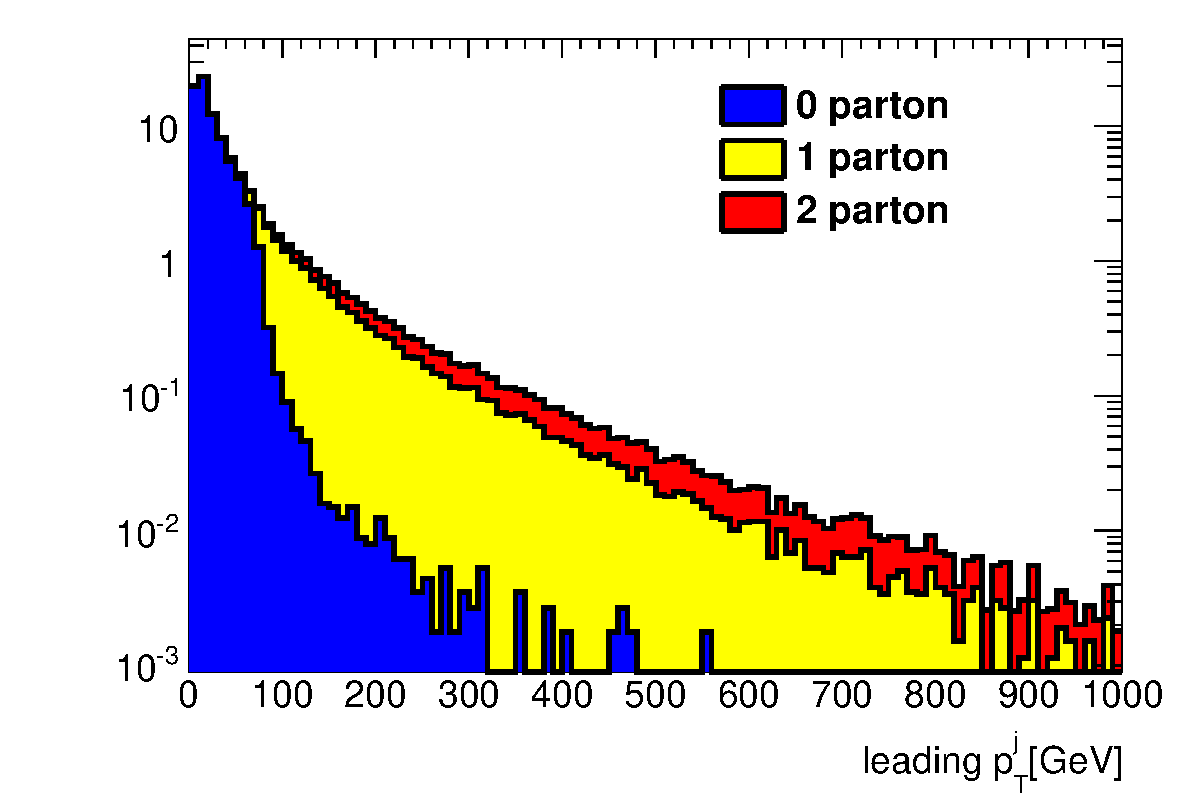
\includegraphics[width=0.95\linewidth]{figures/monojet_appendix/jet1pt_matching80.pdf}
 %	}
 %	\hfill
 %	\subfloat[Transverse momentum of subleading jet]{%
 %    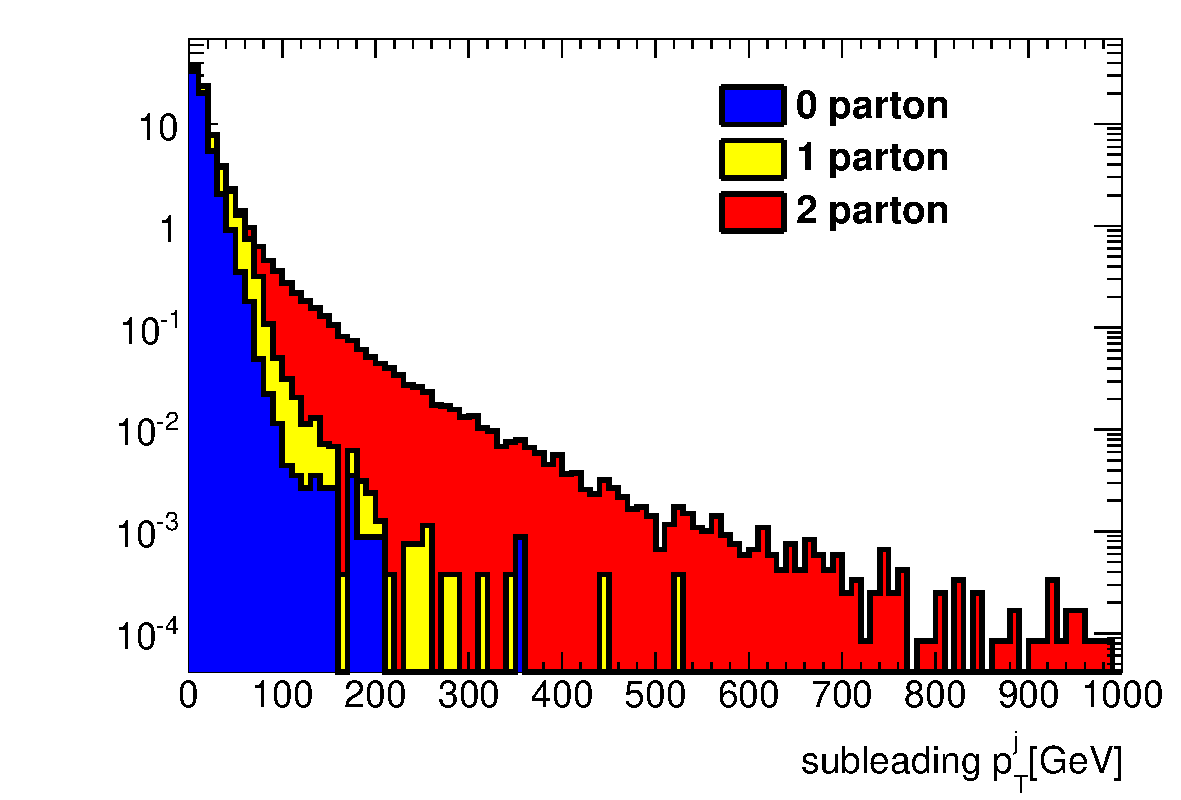
\includegraphics[width=0.95\linewidth]{figures/monojet_appendix/jet2pt_matching80.pdf}
 %	}
 %	\caption{Kinematics distributions for EFT D5 sample with CKKW matching scale at 80 \gev. 0-, 1- and 2-parton emission cases are generated separately and added together by cross sections. The 0-parton emission case has very limited contribution for missing transverse energy larger than 300 \gev region.}
 	\caption{Missing transverse momentum distributions for EFT D5 sample with CKKW-L matching scale at 80\,\gev. Individual contributions from the 0-, 1- and 2-parton emission samples are shown.}
 	\label{fig:Kine_D5_80}
 \end{figure}


In order to describe the signal kinematics correctly and save time during MC production, the parton emissions will only be generated up to a certain multiplicity. The higher multiplicity samples usually have small enough cross sections and the corresponding parts of the phase space can be sufficiently approximated by parton showering in \pythiaEight.
A dedicated study comparing samples generated with up to 1-, 2-, or 3-parton multiplicities was performed, using again the settings for the CKKW-L $k_T$-merging with the 80\,\gev matching scale and the \texttt{Merging:nJetMax} parameter adjusted accordingly.
Figure\,\ref{fig:RatioKine_D5} shows the \MET distribution of the samples at $\MET>250\,\gev$.

%While there is a $\sim10\%$ difference observed between the samples with up to 1 parton and up to 3 partons at low $\MET$, only marginal difference is seen between the samples generated with up to 2 and 3 partons.

%With an event selection requiring \MET and the leading jet \pT being larger than $250\,\gev$ and allowing for up to 3 jets with $\pT>30\,\gev$, the sample generated with up to 1 parton has 17.4\% smaller yield compared to the sample with up to 3 partons, while the yield of the sample with up to 2 partons is only 2.2\% smaller.
With an event selection requiring \MET and the leading jet \pT being larger than $250\,\gev$, the sample generated with up to 1 parton has 10.3\% larger yield compared to the sample with up to 3 partons, while the yield of the sample with up to 2 partons is only 2.3\% larger.
If an additional cut is applied allowing for up to 3 jets with $\pT>30\,\gev$, the agreement improves to 3.2\% larger for up to 1 parton and 0.7\% larger for up to 2 partons, compared with up to 3 partons.
%Note the jet multiplicity cut is important here as the agreement between the two samples improves at higher \MET when the cut is not applied.
%At \MET>400\,\gev$, 0+1 parton emission has 16.8\% yield less and 0+1+2 parton emission has 2.4\% less compared to 0+1+2+3 parton emission. With $\MET>600\,\gev$, 0+1 parton emission has 16.5\% yield less and 0+1+2 parton emission has 2.9\% less compared to 0+1+2+3 parton emission. The same numbers hold if a symmetric cut is added on leading jet transverse momentum.
A similar comparison is shown in Fig.\,\ref{fig:RatioKine_D5_2} for the jet multiplicity in the events with the leadning jet $\pT>250\,\gev$, where an agreement at the level of $\sim3\%$ between the samples with up to 2 and 3 parton emissions is observed for number of jets up to 7.
This justifies it is sufficient to produce samples with up to 2 parton emissions only at the generator level and ignore generating higher parton emissions.


\begin{figure}[h!]
	\centering  
	\subfloat[No jet multiplicity cut]{%
		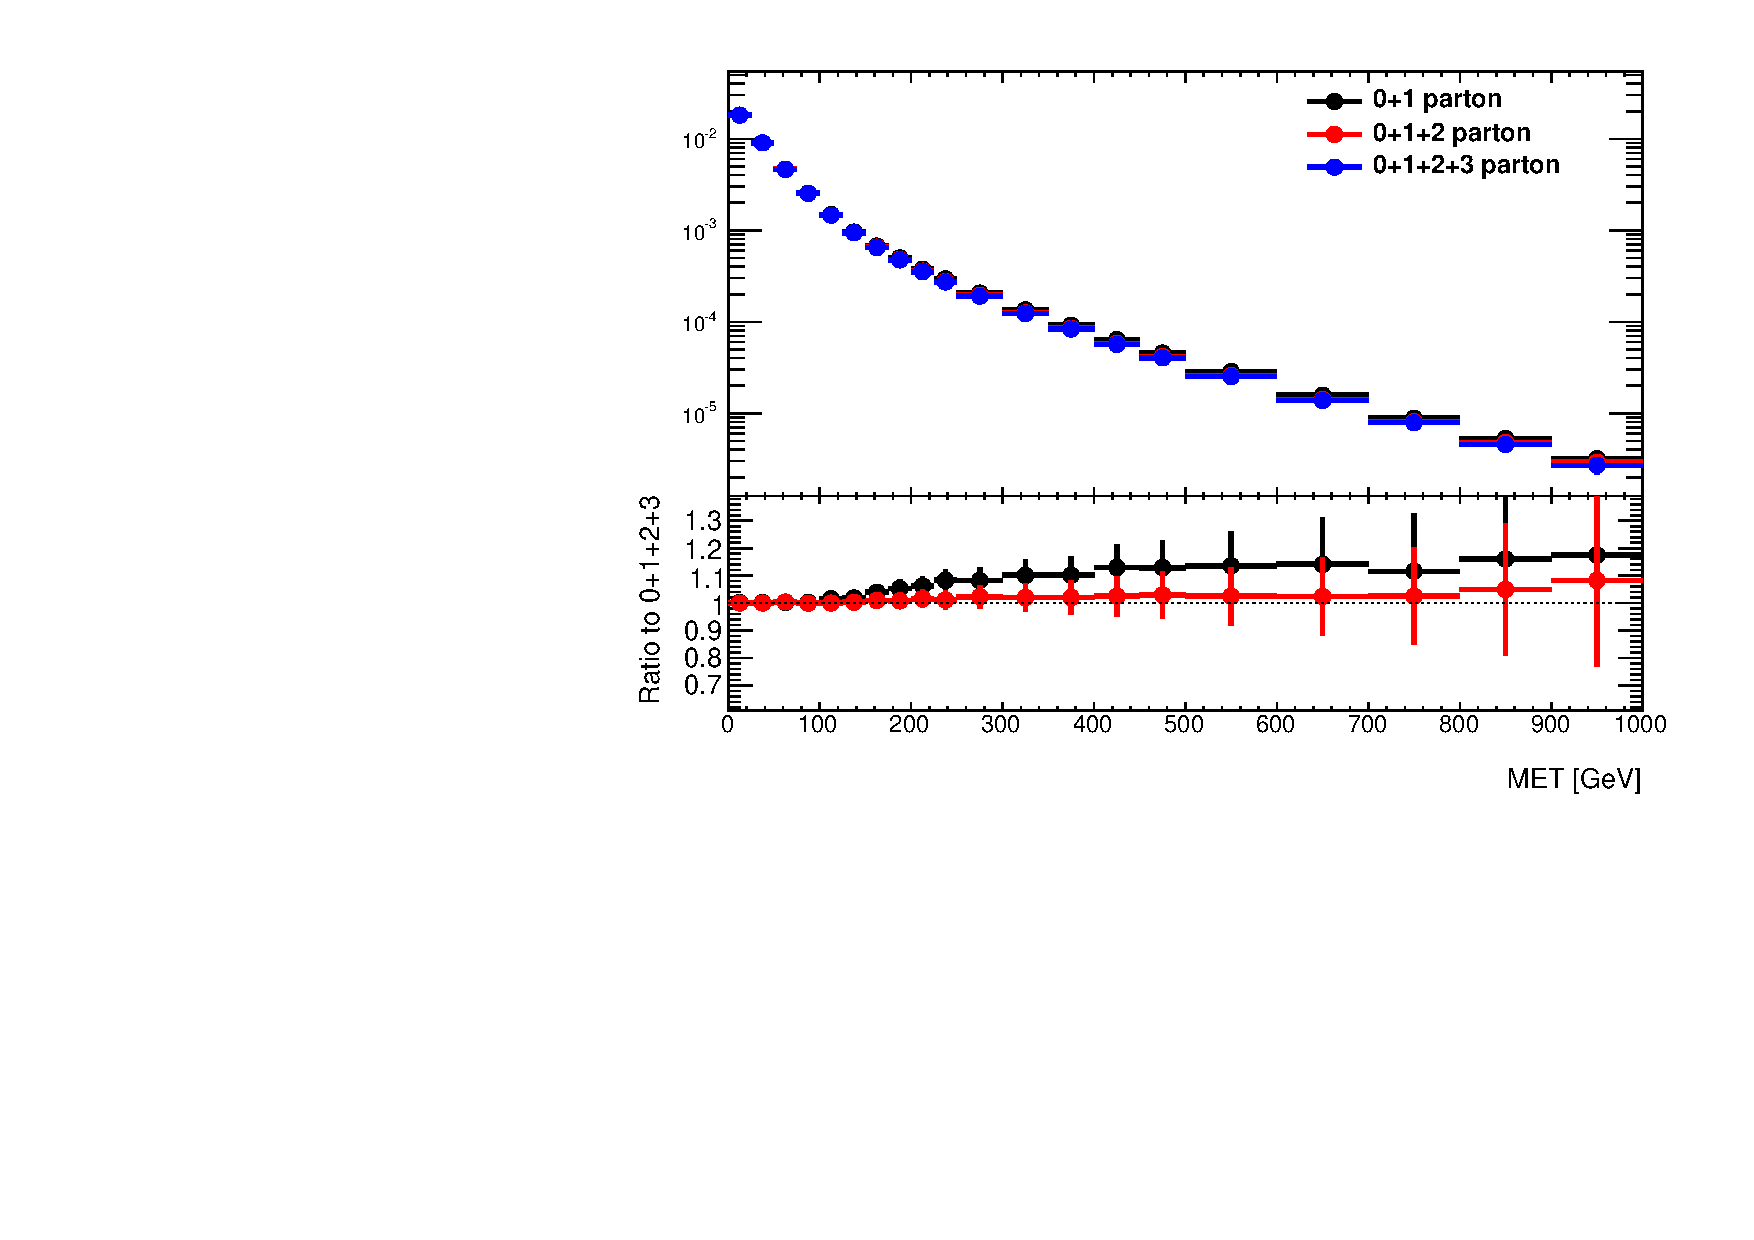
\includegraphics[width=0.95\linewidth]{figures/monojet_appendix/h_MET.pdf}
	}
	\hfill
	\subfloat[$N_{\text{jet}}\leqslant$3]{%
		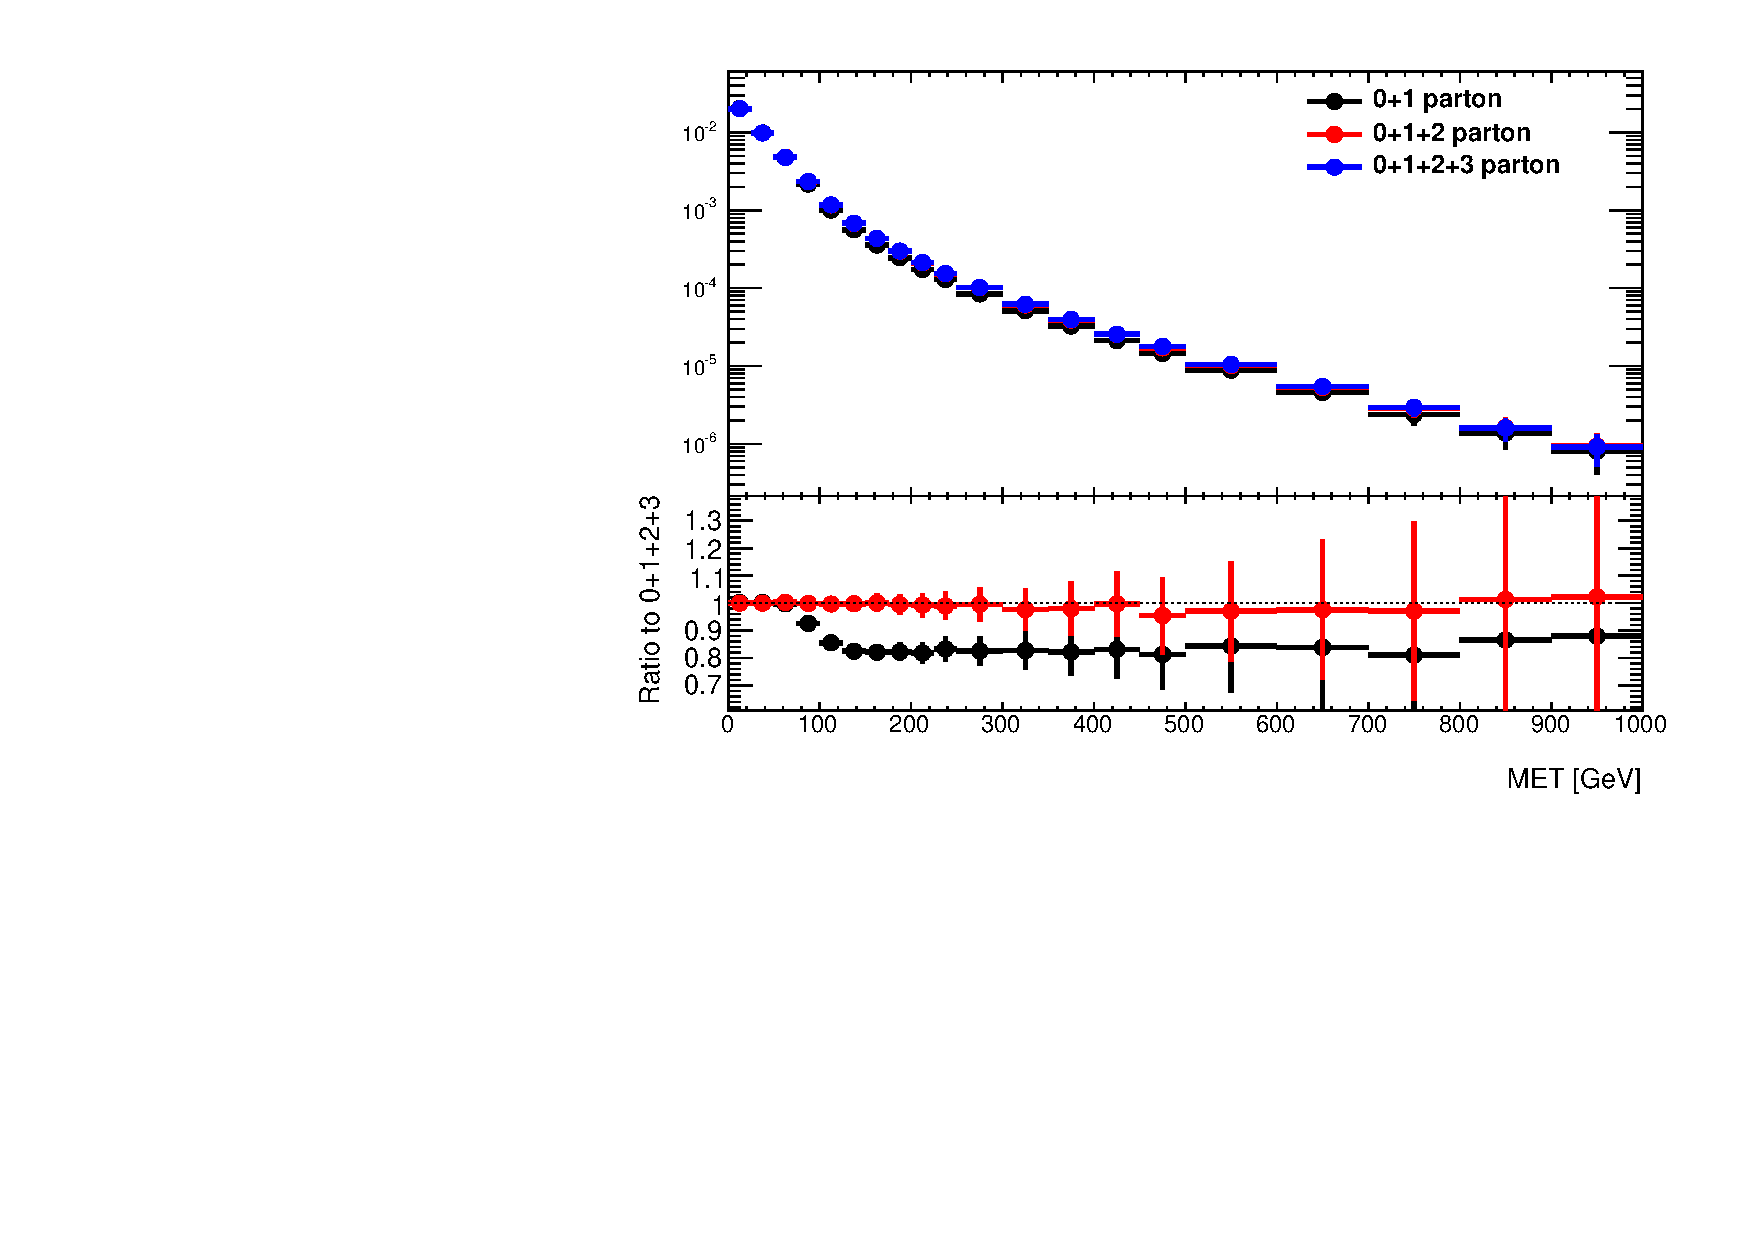
\includegraphics[width=0.95\linewidth]{figures/monojet_appendix/h_MET_3jet.pdf}
	}
	\hfill
%	\subfloat[Transverse momentum of subleading jet]{%
%		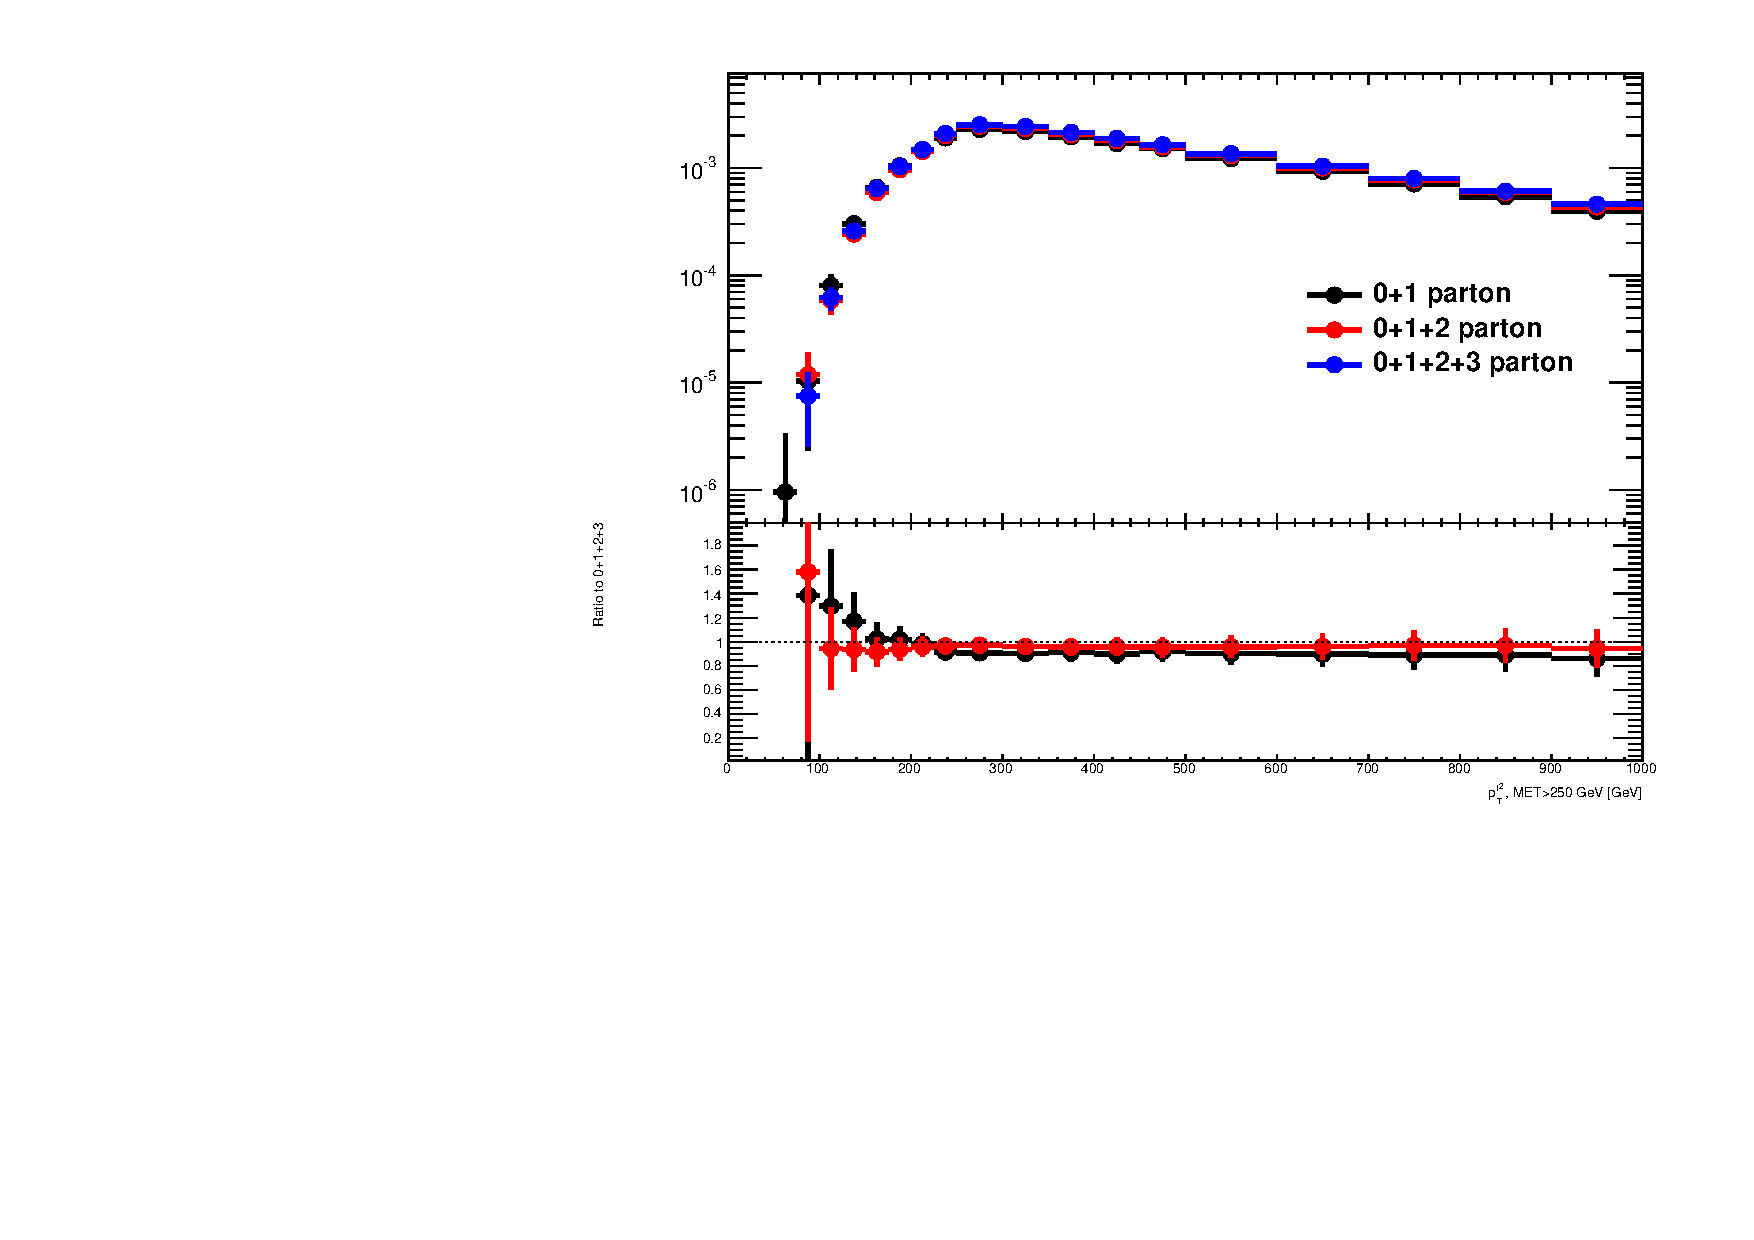
\includegraphics[width=0.95\linewidth]{figures/monojet_appendix/h_pt2_MET250.pdf}
%	}
%	\caption{Kinematics distributions for EFT D5 sample with CKKW matching scale at 80 \gev. 0-, 1-, 2- and 3-parton emission cases are generated separatedly and added together by cross sections.}
	\caption{Missing transverse momentum distributions for EFT D5 sample with CKKW-L matching scale at 80\,\gev produced with maximum 1 (black), 2 (red) and 3 (blue) partons emitted at the generator level. The ratios are shown with respect to the latter sample.}
	\label{fig:RatioKine_D5}
\end{figure}


\begin{figure}[h!]
	\centering  
%	\subfloat[Jet multiplicity, leading jet $p_{T}>30$ \gev]{%
%    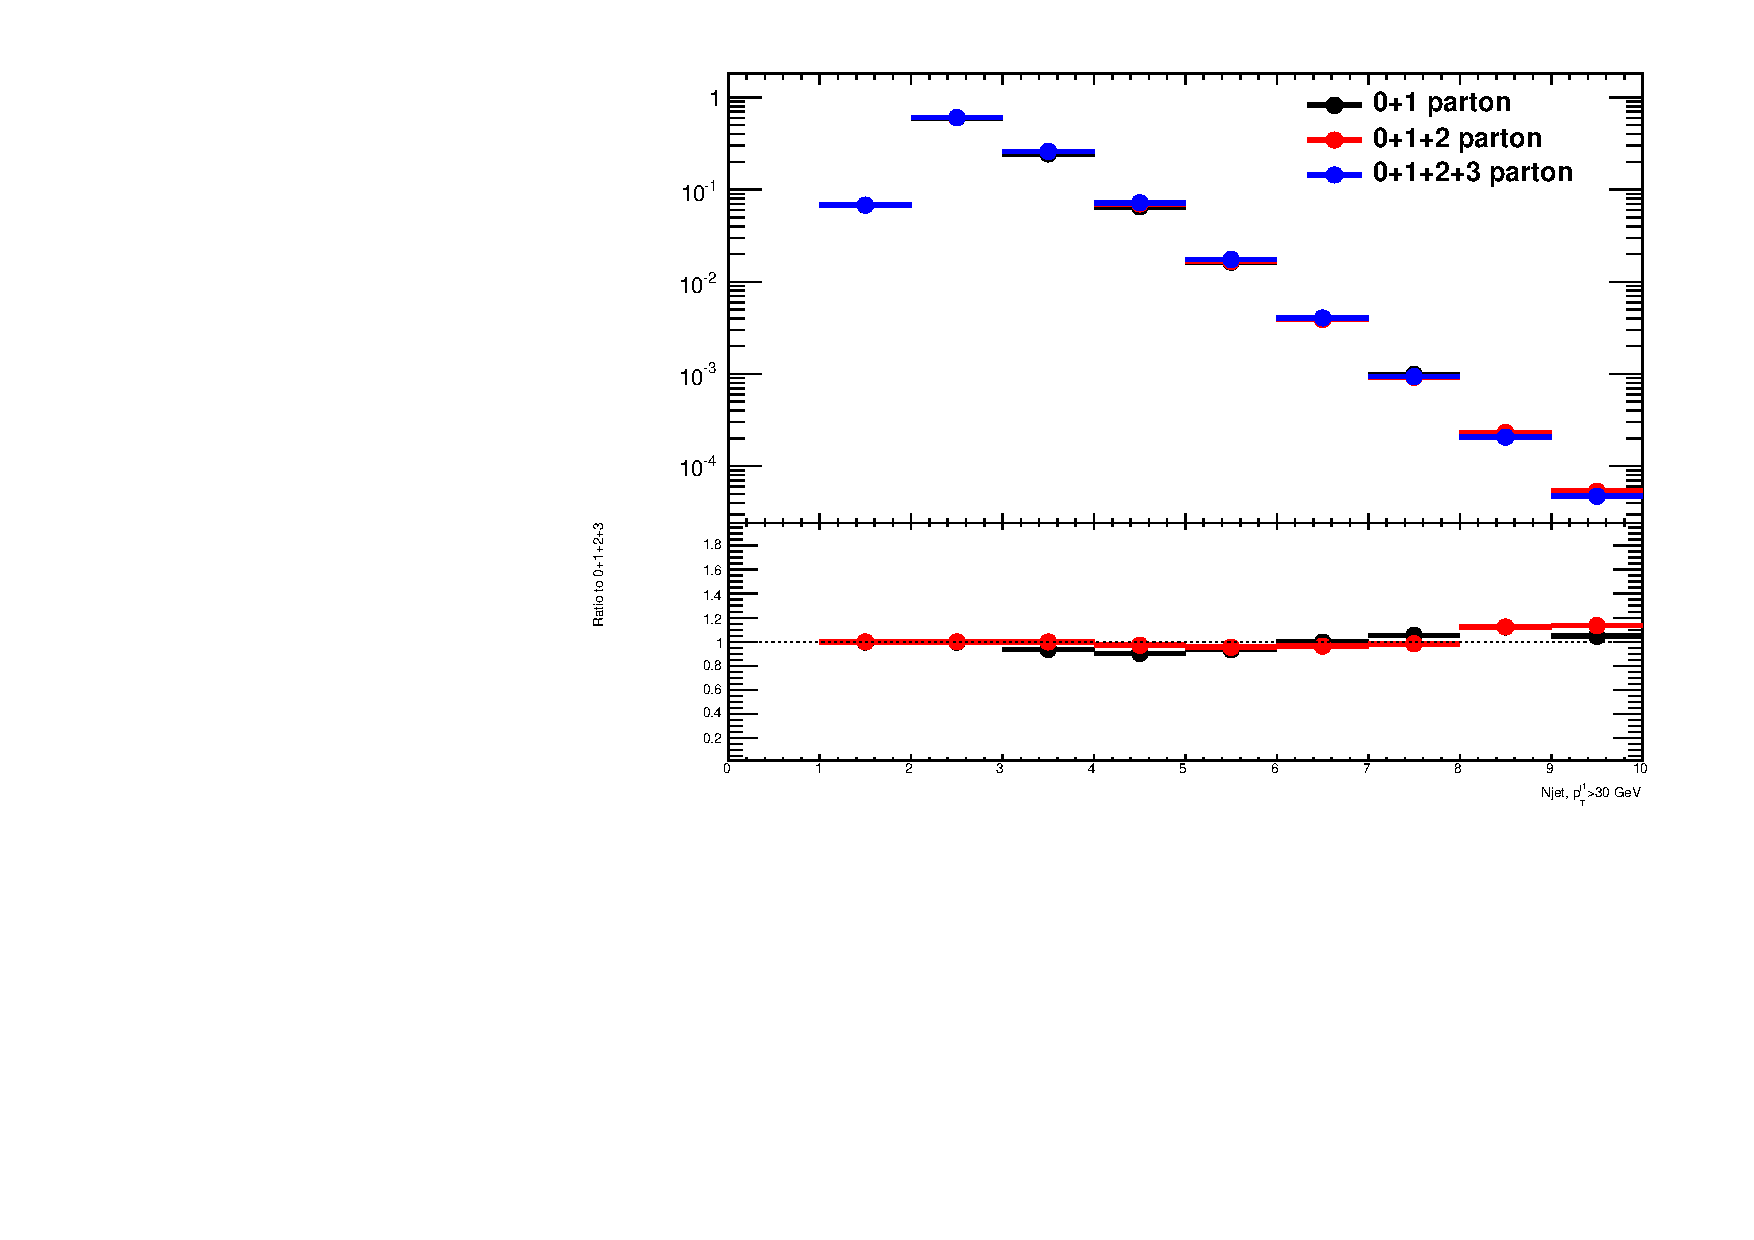
\includegraphics[width=0.95\linewidth]{figures/monojet_appendix/h_njet30.pdf}
%	}
%	\hfill
%	\subfloat[Jet multiplicity, leading jet $p_{T}>80$ \gev]{%
%    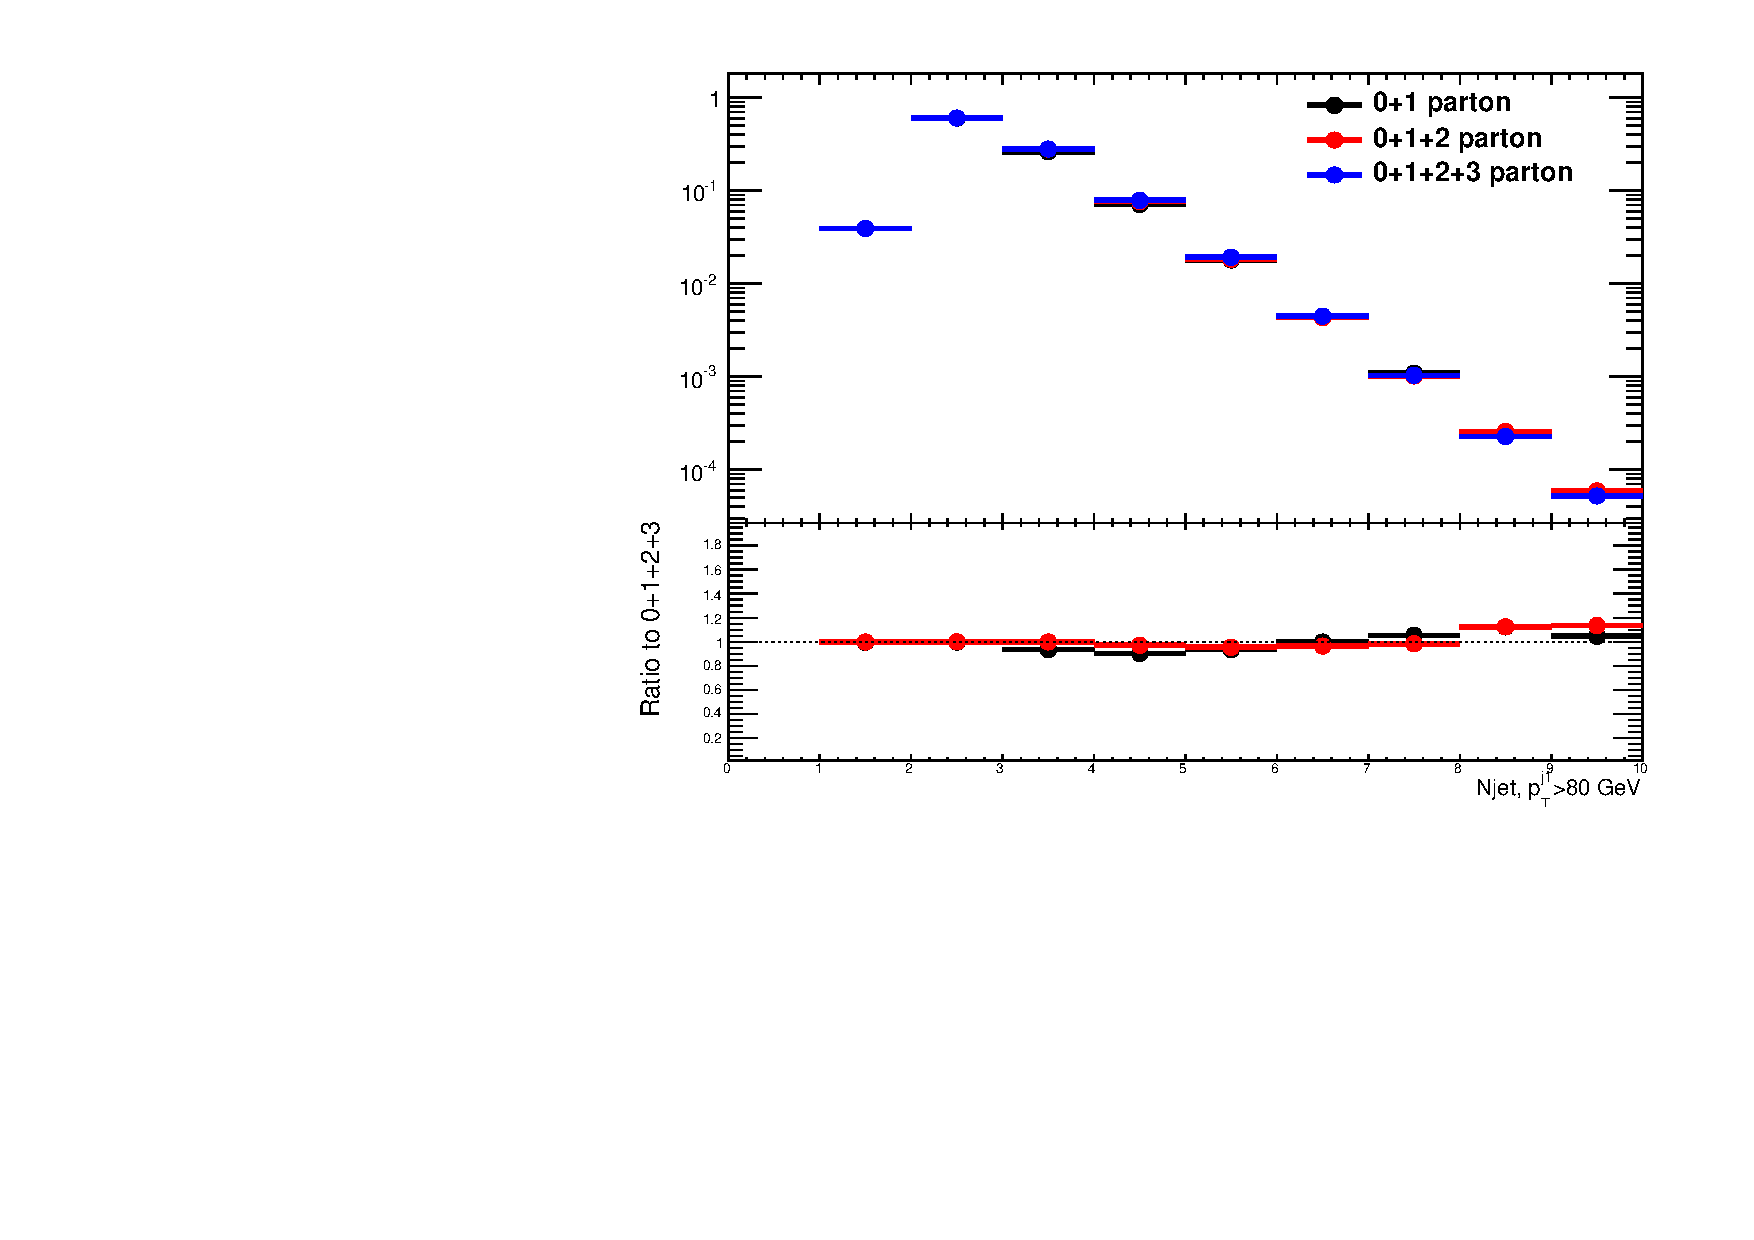
\includegraphics[width=0.95\linewidth]{figures/monojet_appendix/h_njet80.pdf}
%	}
%	\hfill
%	\subfloat[Jet multiplicity, leading jet $p_{T}>250$ \gev]{%
	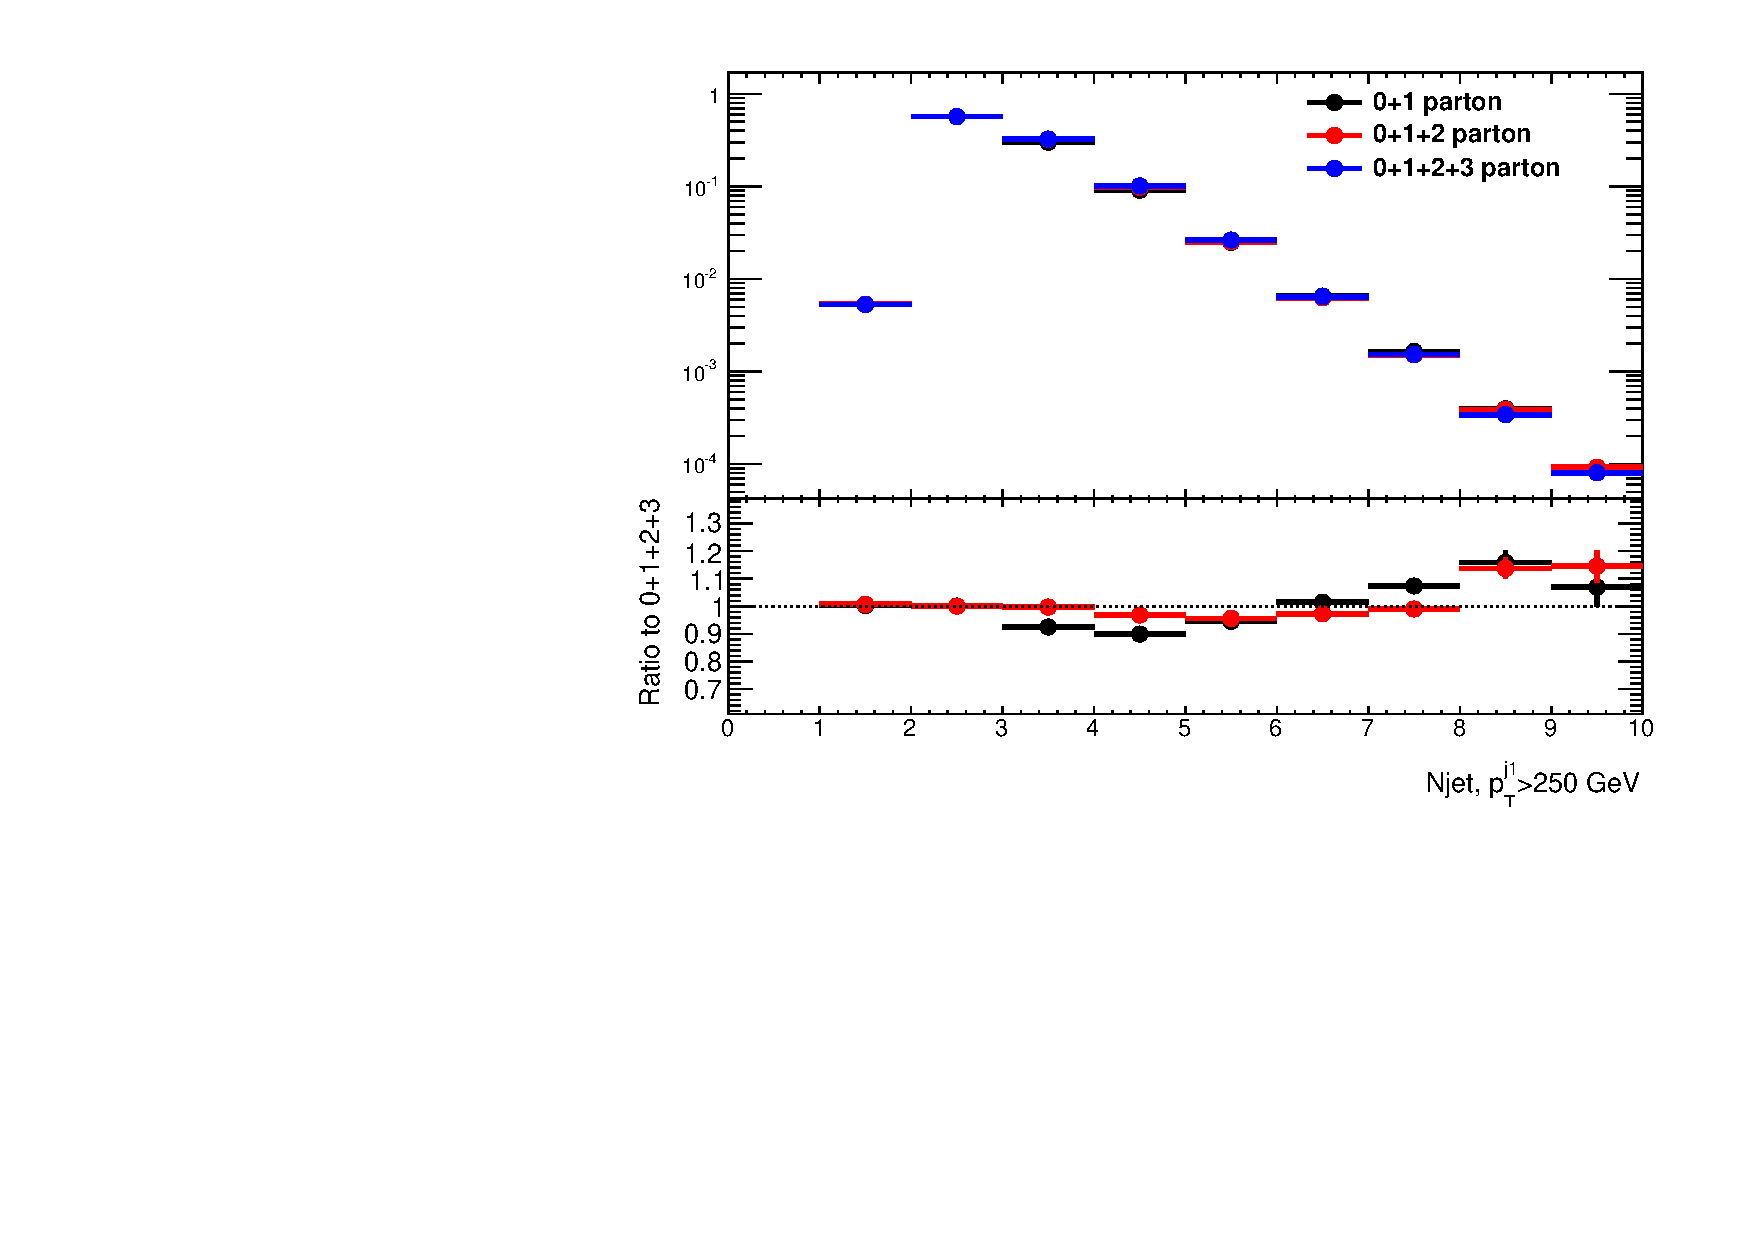
\includegraphics[width=0.95\linewidth]{figures/monojet_appendix/h_njet250.pdf}
%	}
%	\caption{Jet multiplicity distributions for EFT D5 sample with CKKW matching scale at 80 \gev. 0-, 1-, 2- and 3-parton emission cases are generated separatedly and added together by cross sections.}
	\caption{Multiplicity of jets with $\pT>30\,\gev$ and $|\eta|<2.8$ for EFT D5 sample with CKKW-L matching scale at 80\,\gev produced with maximum 1 (black), 2 (red) and 3 (blue) partons emitted at the generator level. The ratios are shown with respect to the latter sample. The leading jet $\pT$ is required to be larger than 250\,\gev.}
	\label{fig:RatioKine_D5_2}
\end{figure}

\subsection{Implementation of \tchannel models for the jet+\MET{} final state}
\label{sec:tchannel_implementation}

The simulations for \tchannel models are available via LO UFO implementations, where events are generated at LO+PS accuracy. The UFO file and parameter cards for the \tchannel models with couplings to light quarks only~\cite{Papucci:2014iwa} can be found on the Forum SVN repository~\cite{ForumSVN_TChannel_PapucciVichiZurek}. The model files from Ref.~\cite{Bell:2012rg} can also be found on the repository~\cite{ForumSVN_TChannel_Amelia}. The latter is the implementation that has been used for the studies in this report: in the monojet case there are only cross section differences between this model and the model in~\cite{ForumSVN_TChannel_PapucciVichiZurek}. 
%while the model from~\cite{Bell:2012rg} has been due to its treatment of boson radiation for the 
 
%~\Todo{This is being checked with the authors.}
Multi-parton simulation and merging are necessary and require particular care for this model: this has not been a topic of detailed studies within the Forum, and we suggest to follow the procedure outlined in Ref.~\cite{Papucci:2014iwa}. 

\subsection{Implementation of \schannel and  \tchannel models with EW bosons in the final state}
\label{sec:EW_implementation}

Currently, simulations for most of these models are available via LO UFO implementations, allowing event generation at the LO+PS accuracy. We note, however, that inclusion of NLO corrections would be possible. In \madgraph, for example, this amounts to simply upgrading the currently employed UFO models to NLO, where the calculations exist for this class of processes. However, this was not available within the timescale of the Forum towards simulation of early Run-2 benchmarks. As a consequence, in this work we have used LO UFO implementations within \madgraph 2.2.3 interfaced to \pythiaEight for the parton shower. The corresponding parameter cards used for the Run-2 benchmark models can be found on the Forum SVN repository~\cite{ForumSVN_EW_DMV}. This is the implementation that will be used for early Run-2 LHC Dark Matter searches.

None of these models requires merging samples with different parton multiplicities  
since the visible signal comes from the production of a heavy SM boson whose transverse momentum distribution is sufficiently 
well described at LO+PS level.  As a result, no special runtime configuration is needed for \pythiaEight. 

\subsection{\texorpdfstring{Implementation of \schannel and \tchannel models with heavy flavor quark signatures}{Simulations for models with heavy flavor quark signatures}}
\label{sec:TTBar_implementation}

Dedicated implementations for DM signals in this final state are available at LO+PS accuracy. 
However, the state of the art of the simulations for $t \bar{t}$ and $b \bar{b}$ with a generic scalar and vector mediator is NLO+PS accuracy. For example, simulations for $t \bar{t}$ + scalar can be obtained via \powheg and {\sc sherpa} starting from the SM implementations. In \madgraph,  all final relevant final states, spin-0 (scalar and pseudo scalar) and spin-1, (vector and axial) are available  at NLO+PS via the dedicated NLO UFO for DM has been released in June 2015~\cite{NewMadgraphModels}).

In the work of this Forum, simulations for the $t \bar{t}$ and $b \bar{b}$ signatures of the scalar mediator model have been 
generated starting from a leading order UFO with \madgraph 2.2.2, using \pythiaEight for the parton shower. 
The UFO file and parameter cards that will be used as benchmarks 
for early Run-2 searches in these final states can be found on the Forum SVN repository~\cite{ForumSVN_DMTTBar}.
Multi-parton merging has been used for the $b \bar{b}$ case but it has not been studied in detail within this Forum. 
The b-flavored DM model of Section~\ref{sec:singleb} is simulated at LO+PS using \madgraph v2.2.3 and \pythiaEight for the parton shower.  
The corresponding UFO and parameter files can be found on the Forum SVN repository~\cite{ForumSVN_DMSingleB}.

\subsubsection{Quark flavor scheme and masses}

In the case of $b \bar{b}$ final state an additional care should be taken when choosing the flavor scheme 
generation and whether quarks should be treated as massive or massless.

The production of DM+$b\bar{b}$, Dark Matter in association with $b$ jets via a decay of a (pseudo) scalar boson, 
is dominated in simplified mediator models by the gluon-gluon initiated production, similar to the production of 
Z+$b\bar{b}$ at the LHC. The Z+$b\bar{b}$ process has been studied in detail in the Z(ll)+$b$-jets final state,  
which can be used to validate both the modeling of DM+bb and, its main background, Z(vv)+$b\bar{b}$. 
In this context, the $p_\textrm{T}$ of the Z boson is related to the observed MET, whereas the $b$-jet kinematics 
determines the ratio of mono-$b$/di-$b$ signatures in the detector.

%suggestion: could add diagrams for Z+bb and Phi+bb production here%

For basic kinematic criteria applied to Z+$b\bar{b}$ production, 
this process leads in $\sim90\%$ of the events to a signature with only 1 $b$-jet in the acceptance (
'Z+1$b$-jet production') and only in  $\sim10\%$ of the events to a signature with 2 $b$-jets in the detector ('Z+2$b$-jets production). 
The production cross section of the Z+$b\bar{b}$ process can be calculated in the 'five-flavor scheme', 
where b quarks are assumed massless, and the 'four-flavor scheme', where massive b quarks are 
used~\cite{Campbell:2003dd,Maltoni:2005wd,Campbell:2005zv}.
Data slightly favour the cross-section predictions in the five-flavor scheme~\cite{Chatrchyan:2014dha} for the 1 $b$-jet signature. 
In this document we have preferred the 5-flavor scheme due to its simplicity and 
cross sections and models in the 5-flavor scheme are available in the repository. 
The PDF used to calculate these cross section is NNPDF3.0 (lhaid 263000). 

On the other hand, both data~\cite{Chatrchyan:2014dha,Chatrchyan:2013zja,CMS:2015mba} 
and theoretical studies~\cite{Frederix:2011qg,Wiesemann:2014ioa} suggest that the best modelling of  an 
inclusive Z+$b\bar{b}$ sample especially for what concerns $b$-quark observables, is achieved at NLO+PS using a 4-flavor scheme 
and a massive treatment of the $b$-quarks.  
In Figure~\ref{fig:4Fvs5F} we show that, at LO, as expected, no appreciable difference is visible in the kinematics between 
either flavor scheme used for DM+$b\bar{b}$. In our generation we have used  NNPDF3.0 set (lhaid 263400).

%Table~\ref{tab:xsec_dmbb_g1} gives the production cross sections for all recommended samples with $g_\textrm{DM}=g_\textrm{SM}=1$.

% We recommend to use in the generation NNPDF3.0 set (lhaid
%263400).
%In the $t bar t$ case we provide 
%values for the suggested coupling scan. 

\begin{figure}[h!]
\begin{minipage}{0.49\textwidth}
	\centering 
	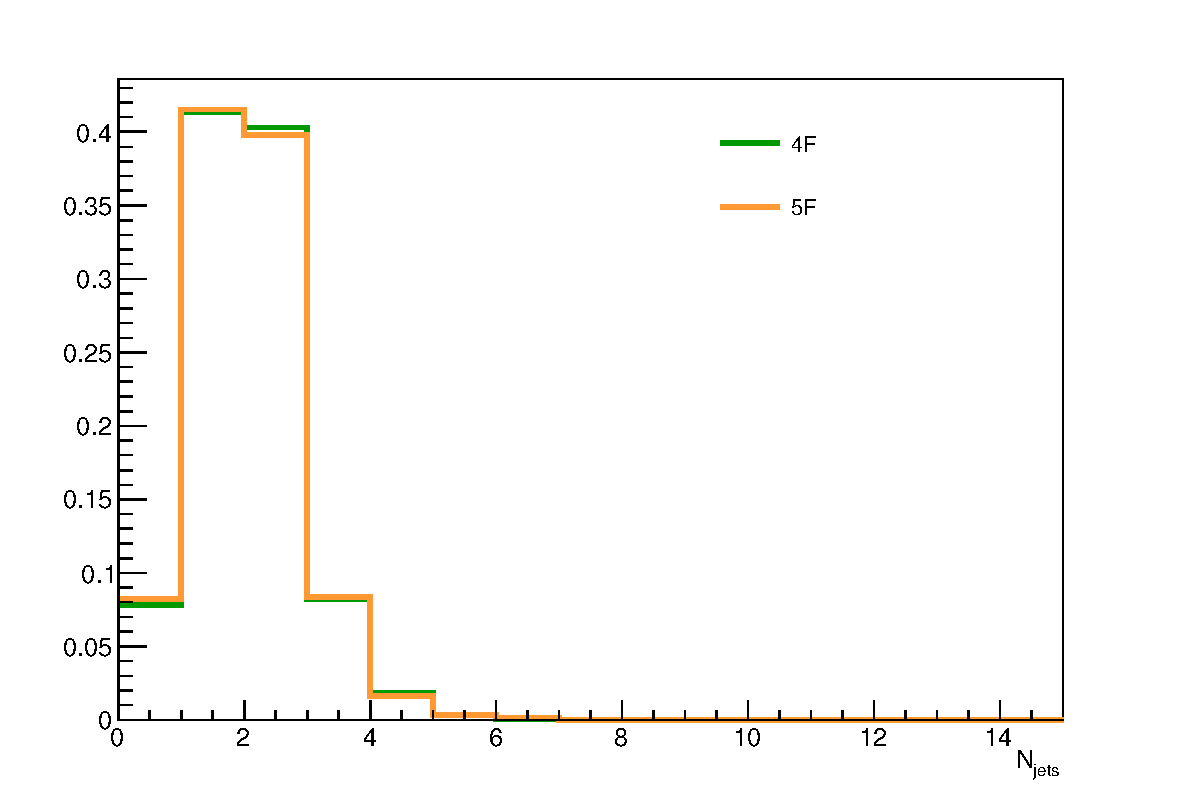
\includegraphics[scale=0.32]{figures/bbar/4Fvs5F_plots/Njets}
\end{minipage}
\hfill
\begin{minipage}{0.49\textwidth}
	\centering 
	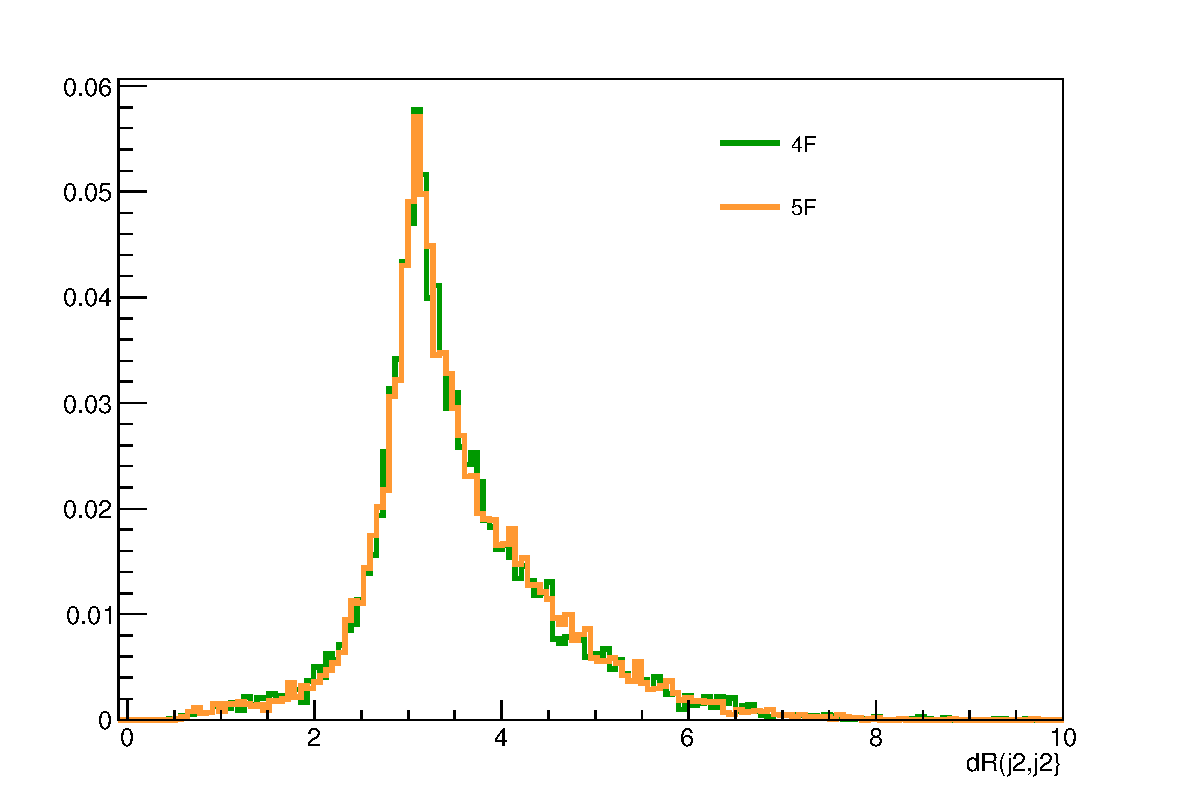
\includegraphics[scale=0.32]{figures/bbar/4Fvs5F_plots/dR12}
\end{minipage}
\caption{Comparison of the jet multiplicity (left) and angular correction $\Delta R(j_1, j_2)$ (right) for the DM+$b\bar{b}$ scalar model generated in the 4-flavor and 5-scheme.
	The samples are generated for $m_\chi=1$~GeV and $m_\phi=10$~GeV.
	\label{fig:4Fvs5F}}
\end{figure}

\section{\texorpdfstring{Implementation of specific models for $V+\MET$ analyses}{Implementation of specific models for V+MET analyses}}

\subsection{Model implementation for mono-Higgs models}
\label{sub:monoHiggs}

Currently, simulations for most of these models are available via LO UFO implementations, allowing event generation at the 
LO+PS accuracy. We note, however, that the inclusion of NLO corrections would be possible but not available in time for the conclusion of these studies. In \madgraph, for example, this amounts to simply upgrading the currently employed UFO models to NLO. Simulation of  loop-induced associated production of DM and Higgs is also possible with the exact top-quark mass dependence. In \madgraph, for example, this can be obtained from the NLO UFO SM and 2HDM implementations. 

In this work all three Higgs+\MET models have been generated at leading
order with \madgraph 2.2.2, using \pythiaEight for the parton shower. No merging procedure has been employed.
The LO UFO implementations of the scalar and vector models that will be used as early Run-2 benchmarks can be found on the Forum SVN  
repository~\cite{ForumSVN_EWMonoHiggs}, while the 2HDM model can be found at this link~\cite{ForumSVN_EWMonoHiggs_2HDM}.

As a final technical remark, we suggest always to let the shower program handle the  $h$ decay 
(and therefore to generate a stable $h$ at the matrix element level).  
In so doing a much faster generation is achieved and the $h$ branching ratios are more accurately 
accounted for by the shower program. 

\subsubsection{\madgraph details for scalar mediator Higgs+MET model}

The case of the associated production of a Higgs and scalar mediator via a top-quark loop can be either considered 
exactly or via an effective Lagrangian where the top-quark is integrated out. While this latter model has 
been shown not to be reliable~\cite{Haisch:2012kf,Hespel:2014sla,Baur:1989cm}, for simplicity we have chosen to perform
the study in this tree-level effective formulation. A full study of the process including
finite top-quark mass and parton shower effects is possible yet left for future work.

\subsubsection{\madgraph details for 2HDM Higgs+MET model}
\label{sec:monoHImplementation}

While a 2HDM UFO implementation at NLO accuracy to be used with \madgraph has been made available at the end of the work
of the Forum~\cite{NewMadgraphModels}, in this work we have only considered LO simulations.%~\Todo{Not sure this is available yet?}
  
The two couplings that can be changed in the implemented model follow the nomenclature below:
 \begin{itemize}
 	\item \texttt{Tb} - $\tan \beta$
 	\item \texttt{gz} - $g_z$, gauge coupling of \Zprime to quarks
 \end{itemize}
 The other couplings are not changed, including \texttt{gx} (the $A \bar \chiDM \chiDM$ coupling) which has little impact on the signal. 
 $\sin \alpha$ is fixed internally such that $\cos (\beta-\alpha) = 0$. 
 The width of the \Zprime and $A$ can be computed automatically within \madgraph. 
 The couplings here don't affect the signal kinematics, so they can be fixed to default values  and then the signal rates can be scaled appropriately. 
 
The nomenclature for the masses in the implemented model is:
 \begin{itemize}
 	\item \texttt{MZp} - PDG ID 32 - \Zprime
 	\item \texttt{MA0} - PDG ID 28 - $A$
 	\item \texttt{MX} - PDG ID 1000022 - dark matter particle
 \end{itemize}
 
The other masses are unchanged and do not affect the result. 
 Both $\Zprime \to hZ(\bar \nu \nu)$ and  $\Zprime \to hA(\bar \chiDM \chiDM)$ contribute to the final state, scaling
 different with model parameters. We recommend to generate them separately, 
 and then add the two signal processes together weighted by cross sections.
 % These signals should be generated separately since they have different $\tan \beta, M_A$ dependence.  

\subsection{Implementation of EFT models for EW boson signatures}
\label{sub:EFTModels}

The state of the art for these models is LO+PS. NLO+PS can be achieved
as well, but the corresponding implementation is not yet available.
In our simulations we have implemented the models in the corresponding
UFO files and  generated events at LO via \madgraph 2.2.2, using \pythiaEight for the parton shower. 
UFO files and parameter cards that will be used as early Run-2 benchmarks can be found on the Forum SVN repository:~\cite{ForumSVN_EWMonoHiggs} for operators 
with Higgs+MET final states and ~\cite{ForumSVN_EWEFTD7} for $W/Z/\gamma$ final states.
These models do not require merging.
